\documentclass[review,3p]{elsarticle}

\usepackage{mystyle}
\linenumbers

\begin{document}

\begin{frontmatter}

\title{Balancing truncation and round-off errors in FEM: one-dimensional analysis}

 \author[1]{Jie Liu\corref{cor1}}
 \ead{j.liu-5@tudelft.nl}
 \author[1]{Matthias M\"oller}
 \ead{m.moller@tudelft.nl}
 \author[1]{Henk M. Schuttelaars}
 \ead{h.m.schuttelaars@tudelft.nl}
 
 \address[1]{Delft Institute of Applied Mathematics\\ Delft University of Technology\\ Van Mourik Broekmanweg 6, 2628 XE Delft, The Netherlands}
\cortext[cor1]{Corresponding author}

\begin{abstract}
In finite element methods, the accuracy of the solution cannot increase indefinitely since the round-off error related to limited computer precision increases when the number of degrees of freedom (DoFs) is large enough. Because a priori information of the highest attainable accuracy is of great interest, we construct an innovative method to obtain the highest attainable accuracy given the order of the elements.
In this method, the truncation error is extrapolated when it converges at the asymptotic rate, and the bound of the round-off error follows from a generically valid error estimate, obtained and validated through extensive numerical experiments. The highest attainable accuracy is obtained by minimizing the sum of these two types of errors.
We validate this method using a one-dimensional Helmholtz equation in space. 
It shows that the highest attainable accuracy can be accurately predicted, and the CPU time required is much smaller compared with that using successive grid refinement. 
\end{abstract}

\begin{keyword}
Finite element method, a posteriori error estimation, optimal number of degrees of freedom, $hp$-refinement strategy, round-off error.
\end{keyword}

\end{frontmatter}

\section{Introduction}

Many problems in engineering sciences and industry are modelled mathematically by initial-boundary value problems comprising systems of coupled, nonlinear partial and/or ordinary differential equations. These problems often consider complex geometries, with initial and/or boundary conditions that depend on measured data \cite{Kumar2016}. 
In some applications, not only the solution, but also its derivatives are of interest \cite{Kumar2016,carey1982derivative}.
For many problems of practical interest, analytical or semi-analytical solutions are not available, and hence one has to resort to numerical solution methods, such as the finite difference, finite volume, and finite element methods. The latter will be adopted throughout this paper and applied to one-dimensional boundary value problems.

The accuracy of the numerically obtained solution is influenced by many sources of errors \cite{ferziger2012computational}: firstly, modelling errors in the set-up of the models, such as the simplification of realistic domains and governing equations and the approximation of initial and boundary conditions; next, truncation errors due to the discretization of the computational domain and the use of basis functions for the function spaces defined on it; then, round-off errors due to the adoption of finite-precision computer arithmetics, rather than exact arithmetics; finally, iteration errors resulting from the artificially controlled tolerance of iterative solvers. 

One tacitly assumes that most errors are well-balanced and/or negligibly small. In this paper, the focus is on the truncation error ($E_{\rm T}$) and the round-off ($E_{\rm R}$), by considering idealized problems, which do not introduce modelling errors, and using a direct solver, which avoids the introduction of iterative errors. In particular, the round-off error is often ignored based on the argument that it will be `sufficiently small' if just IEEE-754 double-precision floating-point arithmetics \cite{zuras2008ieee} are adopted. Therefore, to improve the accuracy, i.e. to decrease $E_{\rm T}$, one often reduces the mesh width ($h$-refinement), increases the approximation order ($p$-refinement), or applies both strategies simultaneously ($hp$-refinement) \cite{guo1986hp,gockenbach2006understanding}. 

The common characteristic of these methods is to increase the number of degrees of freedom (DoFs).
However, $E_{\rm R}$ increases with the number of DoFs, and dominates the total error if more and more DoFs are employed \cite{alvarez2012round,Babuska2018Roundoff}. While typically an impractically large number of DoFs is required for $E_{\rm R}$ to dominate the total error if low(est)-order approximations are used, the number can be very small if high-order approximations are adopted, which are nowadays becoming more and more popular. This shift to higher order approximations makes the results more prone to be dominated by round-off errors. Despite this alarming observation, to the authors’ best knowledge, only very few publications address the impact of accumulated round-off errors on the overall accuracy of the final solution or take them into account explicitly in the error-estimation procedure. The general rule of thumb is still to perform as many $h$-refinements as possible considering the available computer hardware.

The aim of this paper is to systematically analyze the influence of the round-off error on the total error when using $h$-refinements for different orders of $p$. Not only the solution but also its first and second derivatives are investigated for one-dimensional, second order model problems, assuming the second derivative exists in the weak sense \cite{necas2011direct}. Both the standard finite element method (FEM) and the mixed FEM \cite{boffi2013mixed} are analyzed for multiple $p$'s. Furthermore, the following factors are considered: types of boundary conditions and methods of implementing them, choices and configurations of the linear system solver, orders of magnitude of the variables and coefficients. Based on the statistics of the evolution of the round-off error, we propose an algorithm to predict the best accuracy $E_{\rm min}$ that occurs when the sum of $E_{\rm T}$ and $E_{\rm R}$ is the smallest, and the corresponding number of DoFs ($N_{\rm opt}$).

The paper is organized as follows. The model problem, finite element formulation and numerical implementation are described in Section \ref{section_model_problem_FEM_formulation_numerical_implementation}. The approach to predicting ${E}_{\rm {min}}$ is illustrated in Section \ref{section_error_evolution_and_prediction}. The statistics on the evolution of the round-off error are given in Section \ref{section_error_constants}. The algorithm for realizing the approach is put forward in Section \ref{section_algorithm}, followed by its validation by a Helmholtz problem in Section \ref{section_validation}. The conclusions are drawn in Section \ref{paragraph on conclusion}.


\section{Model problem, finite element formulation and numerical implementation}	\label{section_model_problem_FEM_formulation_numerical_implementation}

\subsection{Model problem}

Consider the following one-dimensional second-order differential equation:
\begin{equation}
  -\left(d(x) u_x \right)_x + r(x)u(x) = f(x),\qquad x \in I = [0,1],	\label{1d_second_order_differential_equation}
\end{equation}
with $u$ denoting the unknown variable, which can either be real or complex, $f(x) \in L^2 (I)$ a prescribed right-hand side, and $d(x)$ and $r(x)$ continuous coefficient functions.
By choosing $d(x)=1$ and $r(x)=0$, Eq. (\ref{1d_second_order_differential_equation}) reduces to the Poisson equation; for $d(x)>0$ and not constant, the diffusion equation is found when $r(x)=0$, and the Helmholtz equation \citep{haberman2012applied} is found when $r(x) \neq 0$. 
The boundary conditions are $u(x)=g(x)$ on $\Gamma_D$ and $d(x)u_x=h(x)$ on $\Gamma_N$, where $\Gamma_D$ and $\Gamma_N$ are the boundaries where Dirichlet and Neumann boundary conditions are imposed, respectively.

\subsection{Finite element formulation} 	\label{FE formulation}

For convenience, we introduce two inner products \citep{lipschutz2009linear}:
 \begin{subequations}
  \begin{align}
	\langle f_1, \,f_2 \rangle &= \int _I f_1(x) f_2(x) \, dx,	\\
   \langle f_1, \,f_2 \rangle _{\Gamma} &= f_1(x_0) f_2(x_0).
  \end{align}
 \end{subequations}
where $f_1(x)$ and $f_2(x)$ are continuous functions defined on the unit interval $I$, $\Gamma$ denotes the boundary of $I$, and $x_0$ denotes the values of $x$ on $\Gamma$.

\subsubsection{The standard FEM}

The weak form of Eq. (\ref{1d_second_order_differential_equation}) is derived in \ref{derivation_weak_form_SM}. Imposing the Dirichlet boundary conditions strongly, the weak form reads:
\begin{equation}
\centering
\boxed{ 
\begin{aligned}
&\text{Weak~form}~ 1 ~~~~~~~~~\\
&\text{Find $u \in H _D^1 (I)$ such that:} \\
&\langle {\eta} _{ x }, \, du _{ x } \rangle + \langle\eta, \, ru\rangle = \langle\eta, \, f \rangle + \langle\eta, \, hn\rangle_{\Gamma _N} \qquad \forall \eta \in H _{D0}^1 (I),\\
&\text{with} \\
&~~~~~~~~~~~~~H_{D} ^1 (I) = \{t \; | \; t \in H^1 (I), \; t = g \text{ on } \Gamma _D \},  \\
&~~~~~~~~~~~~H_{D0} ^1 (I) = \{t \; | \; t \in H^1 (I), \; t = 0 \text{ on } \Gamma _D\}.\\
\end{aligned}		\label{sm_weak_form_Diri_strong} 
}
\end{equation}
Imposing the Dirichlet boundary conditions in the weak sense \cite{freund1995weakly}, the weak form reads:
\begin{equation}
\centering
\boxed{
\begin{aligned}
&\text{Weak~form}~ 2 ~~~~~~~~~\\
&\text{Find } u \in H ^1 (I) \text{ such that:}\\
& \langle { \eta} _{ x }, \, du_x \rangle + \langle \eta, \, ru \rangle - \langle \eta, \, du_x n \rangle_{\Gamma _D} + \langle \eta _x, \, u n \rangle_{\Gamma _D} - \langle \eta, \, \rho u n \rangle_{\Gamma _D} \\ 
&= \langle \eta, \, f \rangle + \langle \eta, \, h n \rangle_{\Gamma _N} + \langle \eta _x, \, g n \rangle_{\Gamma _D} - \langle \eta, \, \rho g n \rangle_{\Gamma _D} \qquad \forall \eta \in H ^1 (I), \\
&\text{where } \rho \text{ is a } \text{{positive}} \text{ value that serves as the penalty parameter}.
\end{aligned}	\label{sm_weak_form_Diri_weak}}
\end{equation}
In both forms, $\eta$ denotes the test function, $n$ is equal to 1 at $x=1$, and $-1$ at $x=0$; the terms in the right-hand sides consist of information of Neumann boundary conditions which vanishes if no Neumann boundary conditions are prescribed. We approximate $u$ by a linear combination of a finite number of basis functions:
\begin{equation}
 u \approx u_h ^{(p)} = \sum _ {i=1} ^{m} u _{i} \varphi _{i}^{(p)}. \label{sm_u_approx}%
\end{equation}
Here, $p$ is the element degree, $m$ is the number of DoFs, which equals $p \times t + 1$, with $t$ denoting the total number of grid cells; $u_i$'s are the values of $u_h^{(p)}$ at the DoFs; $\varphi _{i}^{(p)}$'s are $C^0$-continuous Lagrange basis functions supported by Gauss-Lobatto points, which feature the Kronecker-delta property, i.e. $\varphi _{i}^{(p)} (x_j)=\delta_{ij}$, with $x_j$ denoting the support point. This type of element will be referred to as $P_p$. Taking $\eta$ equal to $\varphi ^{(p)}_{k},~ k=1, \,2, \, \ldots , \, m$, the resulting linear system of equations reads
\begin{equation}
 A {U} = F,				\label{matrix_equation_std}
\end{equation}
where $A$ is the stiffness matrix, $F$ the right-hand side and $U=[u_1,\,\ldots,\,u_m]^\top$.

\subsubsection{The mixed FEM}

As a first step, we introduce the auxiliary variable
\begin{subequations}
\begin{align}
   v(x) = - d(x)u_x, \label{mm_strong_form_1} 
\end{align}  
allowing Eq. (\ref{1d_second_order_differential_equation}) to be rewritten as
\begin{align}
  -v_x - r(x)u(x) = -f(x).  \label{mm_strong_form_2}
\end{align}	\label{mm_strong_form_block}%
\end{subequations}
The weak form of Eq. (\ref{1d_second_order_differential_equation}) using the mixed FEM, derived in \ref{derivation_weak_form_MM}, is given by:
\begin{subequations}
\begin{empheq}[box=\fbox]{align}
&\text{Weak~form}~ 3 ~~~~~~~~~\notag\\
&\text{Find $v \in H_{N}^1 (I)$ and $u \in L ^2 (I)$ such that:}	\notag\\
& ~~~~~~~\;\langle w, \, d^{-1}v \rangle - \langle w_x, \,  u \rangle = -\langle w, \, g n \rangle_{\Gamma_D} \qquad \forall w \in H_{N0}^1 (I), \label{mm_weak_form_1}\\ 
& ~~~~~~~~~- \langle q, \, v_x \rangle - \langle q, \, ru \rangle = -\langle q, \, f \rangle \qquad \forall q \in L ^2 (I), \label{mm_weak_form_2}	\\
&    \text{with}\notag\\
& ~~~~~~~~~~~~~~~ H_{N} ^1 (I) = \{t \; | \; t \in H^1 (I), \; t = -h \text{ on } \Gamma _N \},  \notag\\
& ~~~~~~~~~~~~~\, H_{N0} ^1 (I) = \{t \; | \; t \in H^1 (I), \; t = 0 \text{ on } \Gamma _N\}.	\notag 
\end{empheq}
\label{mm_weak_form_block}%
\end{subequations}
In this form, $w$ and $q$ denote the test functions of $v$ and $u$, respectively, and $n$ has the same interpretation as before. We approximate $v$ and $u$ by:
\begin{subequations}
 \begin{align}
 v \approx v _h^{(p)} &= \sum _ {i=1} ^{m} v _{i} \varphi _{i}^{(p)},     \label{mm_u_approx}  \\
 u \approx u _h^{(p-1)} &= \sum\limits _ {j=1} ^{p} u _{sj} \psi _{j}^{(p-1)} \text{ in cell }s, \text{ for } s=1,\,2, \, \ldots, \,t, \label{mm_v_approx}
\end{align}	\label{mm_var_approx_block}%
\end{subequations}
where $m$ is the number of DoFs for $v_h^{(p)}$, which is equal to $p \times t + 1$, $v_i$'s are the values of $v_h^{(p)}$ at the DoFs, and $\varphi _{i}^{(p)}$'s are of the same type of basis functions used in Eq. (\ref{sm_u_approx}); $u_{sj}$'s are the values of $u_h^{(p-1)}$ at the DoFs, $\psi _{j}^{(p-1)}$'s are discontinuous Lagrange basis functions, which implies that two independent $u_{sj}$'s have been assigned at the cell interfaces. This pair of elements will be referred to as $P_p/P_{p-1}^{\text{disc}}$. Replacing $w$ and $q$ by $\varphi _{k}^{(p)} , ~{k} = 1, \,2, \, \ldots , \, p \times t + 1, $ and $ \psi _{e}^{(p-1)} ,~ {e} = 1, \,2, \, \ldots , \, p \times t$, respectively, the resulting coupled linear system of equations that has to be solved reads:
\begin{equation}
 \left[ \begin{array}{cc} M & B  \\ B^\top & 0 \end{array}\right] \left[ \begin{array}{cc} {V} \\ {U} \end{array}\right] =\left[ \begin{array}{cc} G \\ H \end{array}\right], \label{matrix_equation_mix}
\end{equation}
where the mass matrix $M$, discrete gradient operator $B$, and its transpose, the discrete divergence operator $B^\top$, comprise the left-hand side; $G$ and $H$ are the components of the right-hand side; $V=[v_1,\,\ldots,\,v_m]^\top$ and $U=[u_{11},\,\ldots,\,u_{1p},\,\ldots,\,u_{t1},\,\ldots,\,u_{tp}]^\top$, respectively.

For the sake of readability, we will drop the superscript ($p$) or ($p-1$) whenever the approximation order is clear
from the context.

\subsection{Numerical implementation}

\subsubsection{Solution technique}

All results are computed in IEEE-754 double precision \cite{zuras2008ieee} using the deal.\rom{2} finite element library \cite{alzetta2018deal}. Unless stated otherwise, the computational mesh is obtained by globally refining a single element that covers the interval $I$, and the Dirichlet boundary conditions are imposed strongly. The former means that, when the solution is real valued, the number of DoFs equals $2^{R} \times p+1$ using the standard FEM and $2 \times 2^{R} \times p+1$ using the mixed FEM, at the $R$th refinement; when the solution is complex valued, the above numbers double since deal.\rom{2} does not provide native support for complex-valued problems and, hence, all components need to be split into their real and imaginary parts.

To compute the occurring integrals, sufficiently accurate Gaussian quadrature formulas are used. 
To solve the systems of equations, the UMFPACK solver \cite{davis2004algorithm}, which implements the multi-frontal LU factorization approach, is used unless stated otherwise. This solver results in relatively fast computations of the problems considered in this paper, and prevents the iteration errors of iterative solvers. The derivatives of the numerical solution, which are $u_{h,x}$ and $u_{h,xx}$ in the standard FEM and only $v_{h,x}$ in the mixed FEM, are computed in the classical finite element manner, e.g. $u_{h,x}=\sum\limits _{i=1}^m u_i\varphi_{i,x}$ yields an approximation to $u_x$ using standard FEM. Note that, each differentiation decreases the element degree by one.

\subsubsection{Error estimation}

For the numerical results $var_h$, where $var$ can be $u$, $u_x$ and $u_{xx}$ of the standard FEM, and $u$, $v$ and $v_x$ of the mixed FEM, the error measured in the $L_2$ norm is used. It is defined as
\begin{subequations}	\label{formula_abs_error}
\begin{align}		\label{formula_abs_error_analytical}
 E_{h} &= {\|var_{h}- {var}_{\rm exc}\|_{2}}
\end{align}
when the exact solution ${var}_{\rm exc}$ is available, and \cite{Runborg2012VerifyingNC}
\begin{align}		\label{formula_abs_error_numerical}
 {\widetilde {E_{h}}} &= {\|var_{h}- {var}_{h/2}\|_{2}}
\end{align}
otherwise,
\end{subequations}
where $var_{h/2}$ is the numerical solution computed on a mesh once refined with grid size $h/2$. 

\subsubsection{Convergence of the solution}

When the number of DoFs is relatively large, but the round-off error does not exceed the truncation error, the error converges at a fixed rate, known as asymptotic convergence rate, of which the value is one order higher than the approximation order \cite{gockenbach2006understanding}. In practice, the convergence rate in the numerical experiments can be calculated from either 
\begin{subequations}	\label{formula_order_of_convergence_block}
\begin{align}
 Q=\log _2 \left( \frac{E_{h}}{E_{h/2}} \right)
 \label{formula_order_of_convergence_analytical_solution}
\end{align}
using Eq. (\ref{formula_abs_error_analytical}), or
\begin{align}
 \widetilde{Q}=\log _2 \left( \frac{\widetilde {E_{h}}}{\widetilde {E_{h/2}}} \right)		\label{formula_order_of_convergence_finer_solution}
\end{align}
using Eq. (\ref{formula_abs_error_numerical}).
\end{subequations}


\section{Approach to predicting the highest attainable accuracy}      \label{section_error_evolution_and_prediction}

A conceptual sketch of $E_h$ against the number of DoFs ($N_h$) in a log-log plot can be found in Fig.~\ref{error_evolution_one_p}, also see \cite{butcher2016numerical}.
When $N_h$ is relatively small ($N_h<N_c$), $E_h$ does not decrease at the aforementioned asymptotic order of convergence, and only when $N_h$ is large enough ($N_c \leqslant N_h < N_{\rm opt}$) this asymptotic order of convergence is attained.  The transition from the first phase, denoted by black circles, to the second phase, denoted by green circles, is usually fast, cf. Fig.~\ref{error_evolution_one_p}. $E_h$ in both phases is controlled by the truncation error $E_{\rm T}$; in the second phase $E_h$ can be represented by 
\begin{equation}
 E_{h} \approx E_{\rm T} = \alpha_{\rm T}{N_{h}}^{-\beta_{\rm T}}.		\label{formula_truncation_error}
\end{equation}
Here $\alpha_{\rm T}$ is the offset, and $\beta_{\rm T}$ is the slope of the line approximating $E_h$, equalling the asymptotic order of convergence, see \ref{proof_slope_ET} for the proof. Note that, $\alpha_{\rm T}$ can be inverted by using 
\begin{equation}
 \alpha_{\rm T} = {E_{\rm c}}/{N_{\rm c}}^{- \beta_{\rm T}},		\label{formula_offset_truncation_error}
\end{equation}
at the beginning of the second phase, where $E_{\rm c}$ equals the corresponding error $E_h$.

When $N_h$ is increased too much ($N_h \geqslant N_{\rm opt}$), the round-off error $E_{\rm R}$ starts to dominate and $E_h$ increases, illustrated by orange circles. At this phase, the slope of the line approximating $E_h$, denoted by $\beta_{\rm R}$, tends to be fixed \cite{Babuska2018Roundoff,WalterFrei}. The parameter $\beta_{\rm R}$ and the associated offset, denoted by $\alpha_{\rm R}$, are investigated in detail in Section \ref{section_error_constants}. As will be shown there, $\alpha_{\rm R}$ and $\beta_{\rm R}$ are fixed constants, which allows us to estimate $E_h$ as
\begin{equation}
 E_{h} \approx E_{\rm R} = \alpha_{\rm R}{N_{h}}^{\beta_{\rm R}}.		\label{formula_round_off_error}
\end{equation}
In summary, the evolution of $E_h$ is described in Table~\ref{phases_error}, and depicted in Fig. \ref{error_evolution_one_p}.

\begin{figure}[!ht]
\centering
   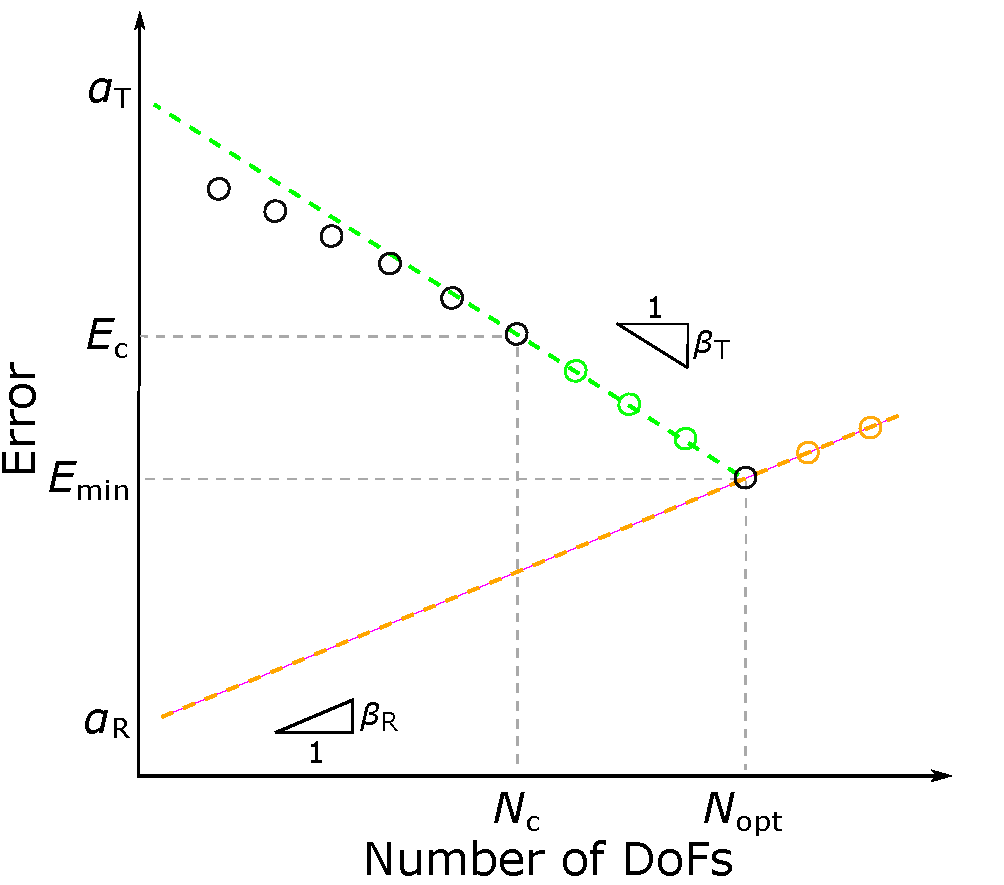
\includegraphics[width=0.5\linewidth]{../2_figure/1_error_evolution_one_p/sketch_error_one_p.pdf}
   \caption{Conceptual sketch of the error evolution against the number of $\text{DoFs}$.}
   \label{error_evolution_one_p}
\end{figure}
 
\begin{table}[!ht]
\small
\caption [sss] {Description of the evolution of $E_h$.}
\label{phases_error}
\centering
 \begin{tabular}{|l|c|c|c|} \hline   
 & 1. {$N_h < N_{\rm c}$} & 2. {$N_{\rm c} \leqslant N_h < N_{\rm opt}$} & 3. {$N_{\rm opt} \leqslant N_h$} \\ \hline
Feature & \makecell[l]{Decreasing but not\\ converging at slope $\beta_{\rm T}$} & \makecell[l]{Decreasing and converging\\ at slope $\beta_{\rm T}$, with the offset $\alpha_{\rm T}$} & \makecell[l]{Increasing and converging\\ at slope $\beta_{\rm R}$, with the offset $\alpha_{\rm R}$} \\	\hline
Dominant error & \multicolumn{2}{c|}{Truncation error} & Round-off error \\	\hline
Formula & - & $E_h \approx E_{\rm T}=\alpha_{\rm T}{N_h}^{-\beta_{\rm T}}$ & $E_h \approx E_{\rm R}=\alpha_{\rm R} {N_h}^{\beta _{\rm R}}$ \\	\hline
\end{tabular}
\end{table}

Since the evolution of $E_{h}$ ($=E_{\rm T}+E_{\rm R}$) is known after entering the second phase, by solving
\begin{equation}
    \frac{d(E_{\rm T}+E_{\rm R})}{dN}=0,    \label{derivative_condition_N_opt}
\end{equation}
we can predict the optimal number of DoFs
\begin{subequations}
\begin{align}
 N_{\rm opt} = \left( \frac{\alpha_{\rm T} \beta_{\rm T}}{\alpha _{\rm R} \beta_{\rm R}} \right)^{\frac{1}{\beta_{\rm T} + \beta_{\rm R}}},
\end{align}
and hence, the highest attainable accuracy is given by
\begin{align}
 E_{\rm min} = \alpha_{\rm T} {N_{\rm opt}}^{- {\beta _{\rm T}}}+\alpha_{\rm R} {N_{\rm opt}}^{{\beta _{\rm R}}}.
\end{align}
\end{subequations}

\section{Results}  	\label{section_error_constants}

In this section, we assess the general values of $\alpha_{\rm R}$ and $\beta_{\rm R}$.
We start with a benchmark Poisson equation, for which the influences of solution strategies and boundary conditions are investigated, and then consider more general parameters for the Poisson equation, as well as the diffusion and Helmholtz equations.

\subsection{Benchmark Poisson equation}		\label{section_preliminary_results}

We consider the Poisson equation with $f(x)=-e^{- (x-1/2)^2} \left({4x^2 - 4x -1} \right)$. The boundary conditions are imposed as follows: $u(0)=u(1)= e^{-1/4}$. The exact solution reads $u(x)=e^{- (x-1/2)^2}$. The error $E_h$ of the resulting solution $u$, and its first and second derivative, using the standard FEM and the mixed FEM, with $p$ ranging from 1 to 5 are in Fig.~\ref{py_bench_Pois_SM} and Fig.~\ref{py_bench_Pois_MM}, respectively. In these figures, $\alpha_{\rm R}$ and $\beta_{\rm R}$ are denoted.

\begin{figure}[!ht]
    \begin{subfigure}{5.5cm}
        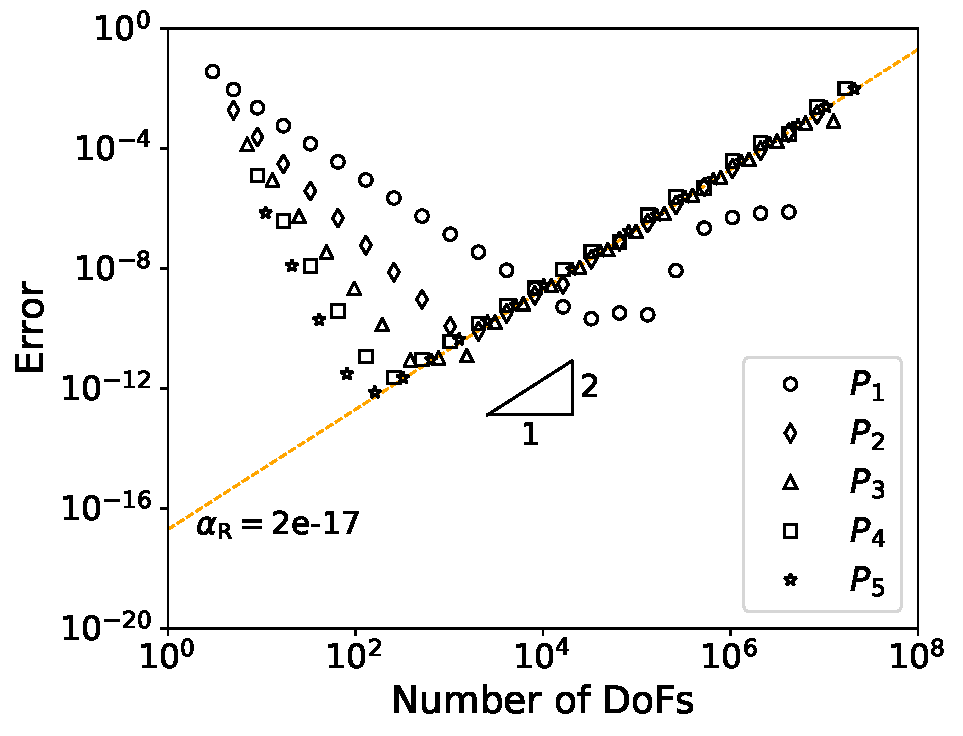
\includegraphics[width=1.0\linewidth]{../2_figure/5_error_plot/py_bench_Pois_SM_solu.pdf}
        \caption{$u$}
        \label{py_bench_Pois_SM_solu}
    \end{subfigure}
    \hspace{-0.2cm}
    \begin{subfigure}{5.5cm}
        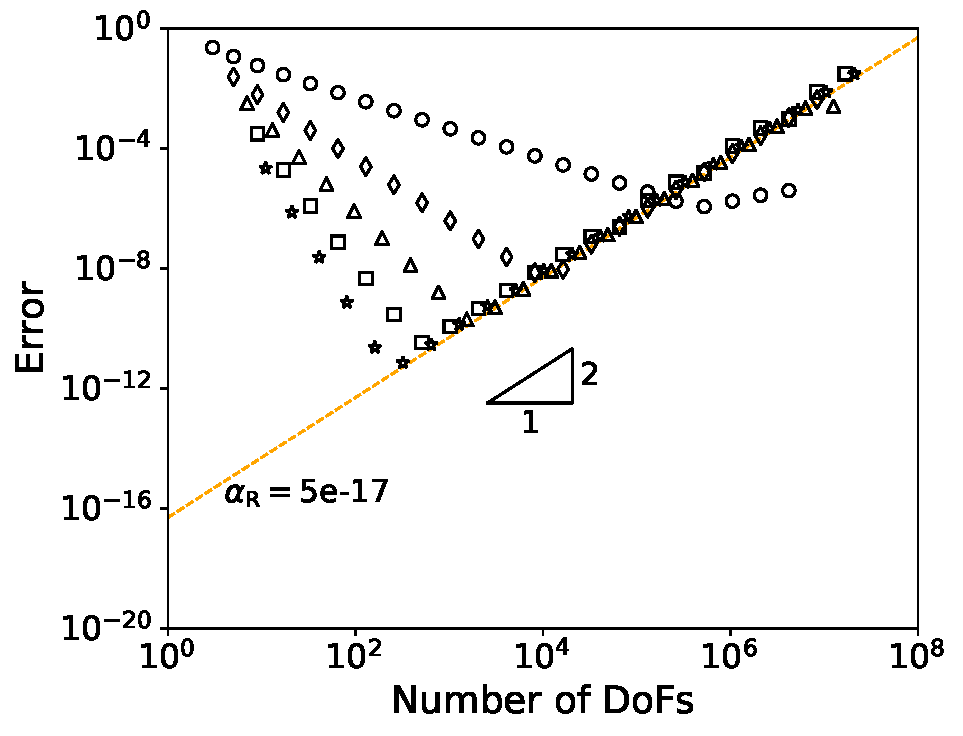
\includegraphics[width=1.0\linewidth]{../2_figure/5_error_plot/py_bench_Pois_SM_grad.pdf}
        \caption{$u_x$}
        \label{py_bench_Pois_SM_grad}
    \end{subfigure}
    \hspace{-0.2cm}
    \begin{subfigure}{5.5cm}
        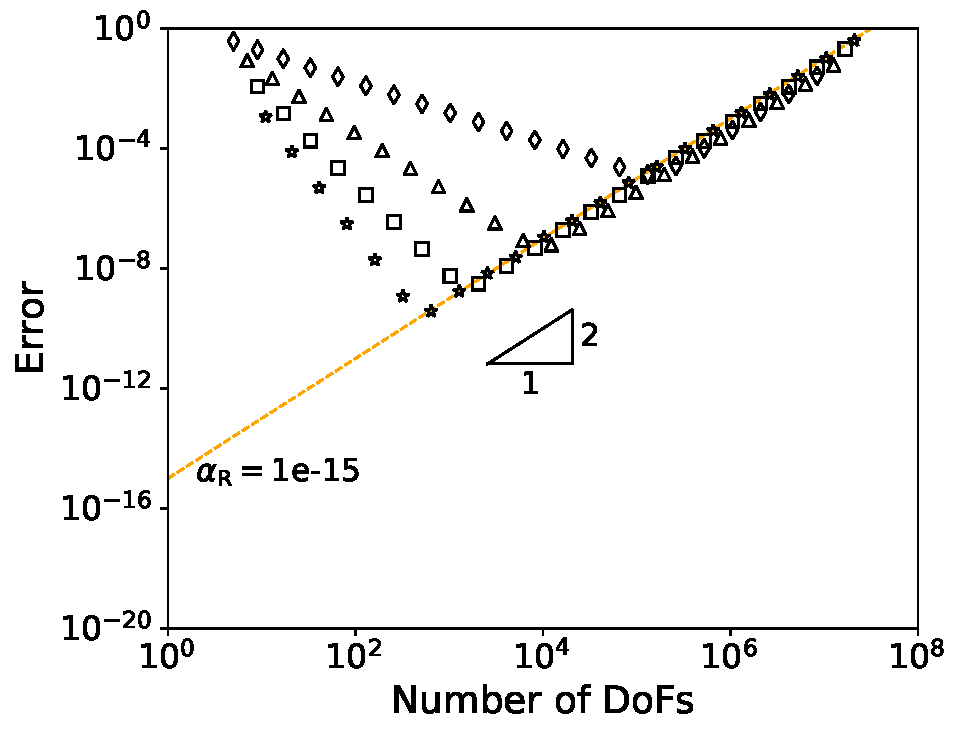
\includegraphics[width=1.0\linewidth]{../2_figure/5_error_plot/py_bench_Pois_SM_2ndd.pdf}
        \caption{$u_{xx}$}
        \label{py_bench_Pois_SM_2ndd}
    \end{subfigure}
\caption{Absolute errors for the benchmark Poisson equation using the standard FEM.}
\label{py_bench_Pois_SM}
\end{figure}

\begin{figure}[!ht]
    \begin{subfigure}{5.5cm}
        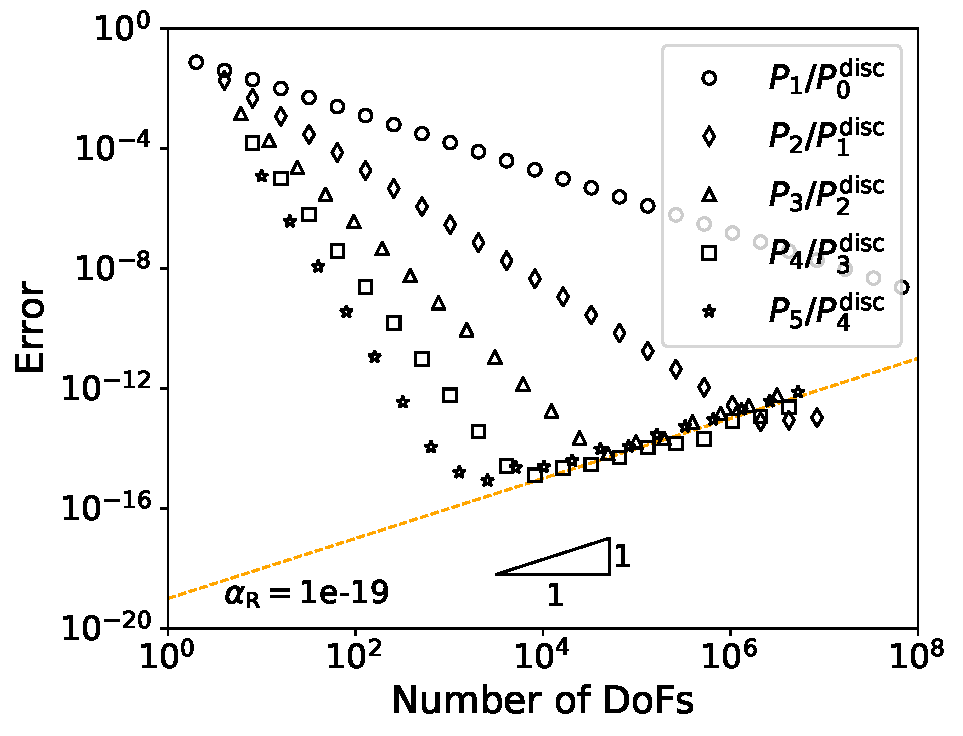
\includegraphics[width=1.0\linewidth]{../2_figure/5_error_plot/py_bench_Pois_MM_solu.pdf}
        \caption{$u$}
        \label{py_bench_Pois_MM_solu}
    \end{subfigure}
    \hspace{-0.2cm}
    \begin{subfigure}{5.5cm}
        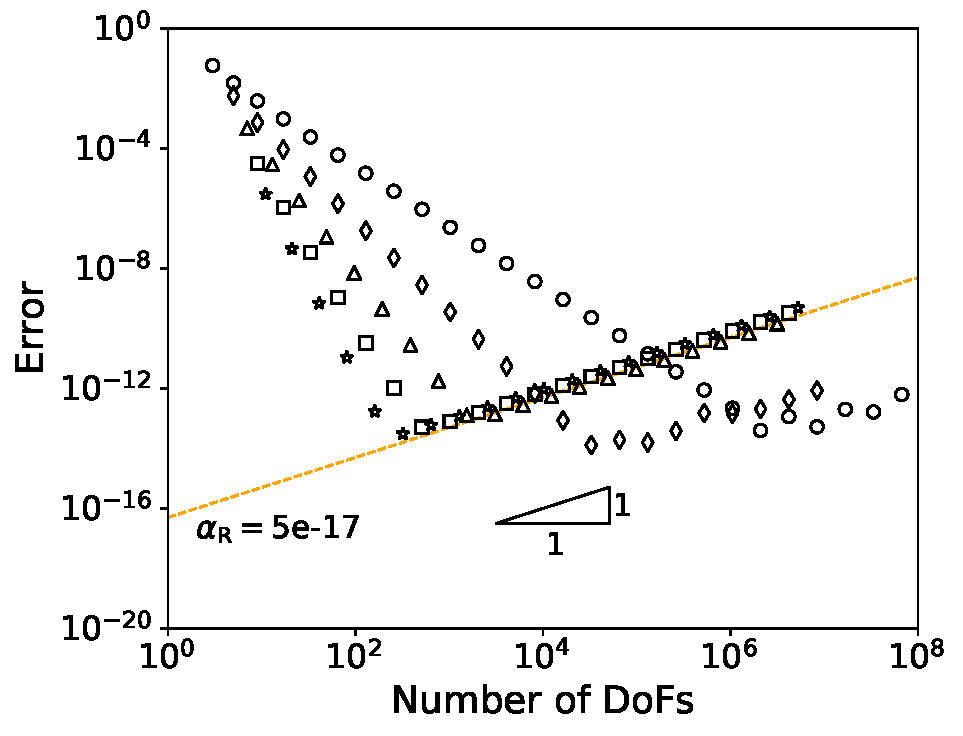
\includegraphics[width=1.0\linewidth]{../2_figure/5_error_plot/py_bench_Pois_MM_grad.pdf}
        \caption{$v$}
        \label{py_bench_Pois_MM_grad}
    \end{subfigure}
    \hspace{-0.2cm}
    \begin{subfigure}{5.5cm}
        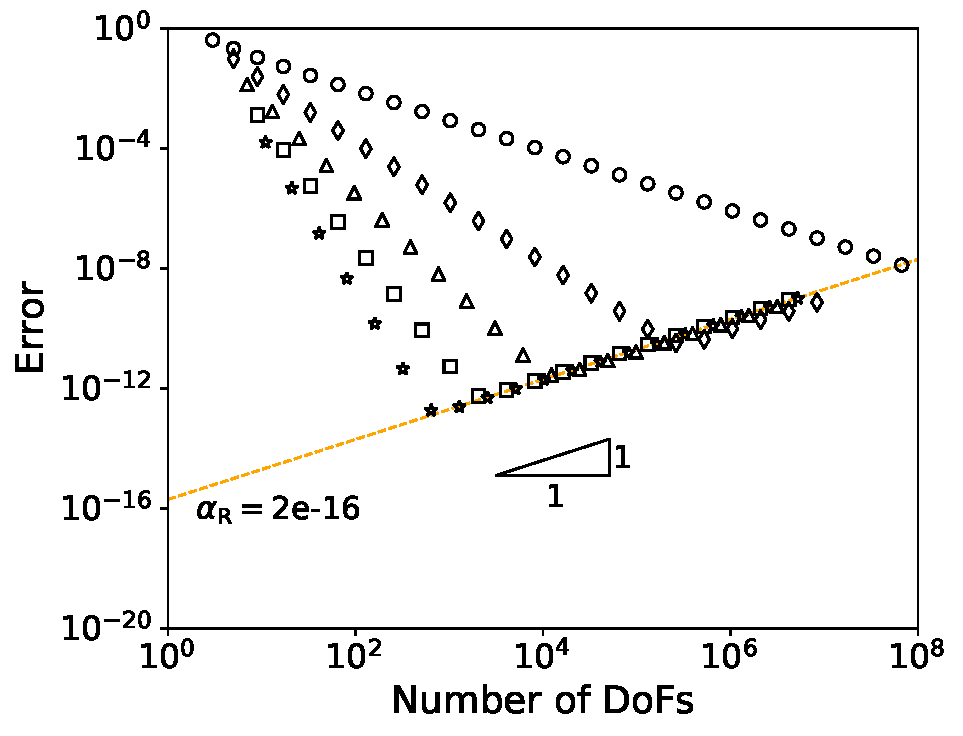
\includegraphics[width=1.0\linewidth]{../2_figure/5_error_plot/py_bench_Pois_MM_2ndd.pdf}
        \caption{$v_x$}
        \label{py_bench_Pois_MM_2ndd}
    \end{subfigure}
\caption{Absolute errors for the benchmark Poisson equation using the mixed FEM.}
\label{py_bench_Pois_MM}
\end{figure}

It is found that, for all dependent variables and their derivatives, the values of $\alpha_{\rm R}$ and $\beta_{\rm R}$ of different element degrees are the same. The statistics of the former can be found in Fig.~\ref{alpha_R_benchmark_Poisson}. The values of $\beta_{\rm R}$ only depend on the FEM method, and are 1 using the mixed FEM and 2 using the standard FEM. Notably, $\alpha_{\rm R}$ is of order $10^{-16}$, which is as expected when using double precision, and tends to increase slightly with increasing order of derivative. Furthermore, $\alpha_{\rm R}$ of the mixed FEM is smaller than that of the standard FEM.  

For larger $p$, $E_{\rm T}$ decreases faster such that smaller ${E}_{\text{min}}$ can be obtained, see Fig.~\ref{E_min_benchmark_Poisson}. In general, smaller $E_{\rm min}$ can be obtained using the mixed FEM compared to using the standard FEM.

\begin{figure}[!ht]
\centering
\begin{subfigure}[b]{0.35\textwidth}
\scalebox{0.85}{
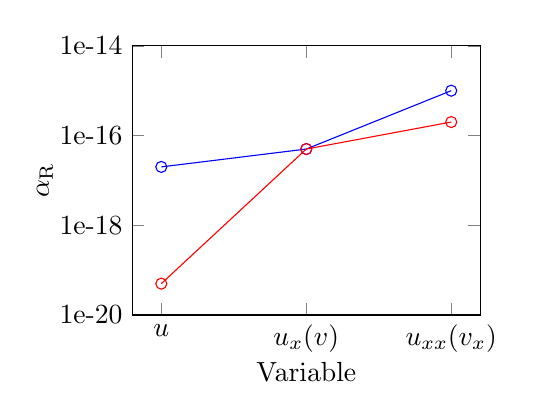
\begin{tikzpicture} 
\begin{axis}
[
    ymode=log,    
    ymin=1e-20,
    ymax=1e-14,
    ytick={1e-20, 1e-18, 1e-16, 1e-14},
    yticklabels={1e-20, 1e-18, 1e-16, 1e-14},      
    legend style={nodes={scale=0.8},at={(0.03,0.85)},anchor=west},
    legend cell align={left},
    height=5cm,
    width=6cm,
    ylabel={$\alpha_{\rm R}$},
	ylabel style={at={(-0.2,0.5)}},     
    xtick={0,1,2,3,4},
    xticklabels={$u$, $u_x(v)$, $u_{xx}(v_x)$},
    xlabel={Variable},
	xlabel style={at={(0.5,-0.14)}}
]
\addplot[blue,mark=o,mark options={color=blue,fill=blue}] coordinates {(0,2.0e-17) (1,5.0e-17) (2,1.0e-15)};
\addplot[red,mark=o,mark options={color=red,fill=red}] coordinates {(0,5.0e-20) (1,5.0e-17) (2,2.0e-16)};
\end{axis}
\end{tikzpicture}
}
\vspace{-0.2cm}
\caption{$\alpha_{\rm R}$}
\label{alpha_R_benchmark_Poisson}
\end{subfigure}
\hspace{-0.7cm}
\begin{subfigure}[b]{0.35\textwidth}
\scalebox{0.85}{
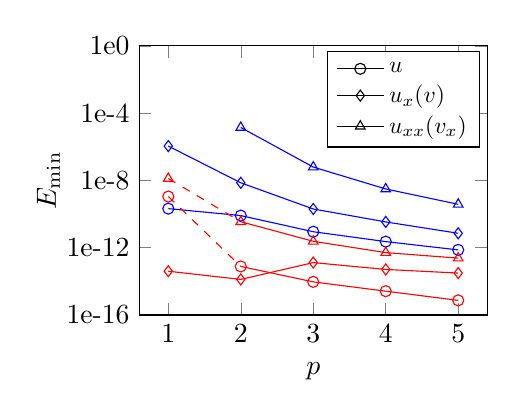
\begin{tikzpicture}
\begin{axis}
[
    ymode=log,    
    ymin=1e-16,
    ymax=1e0,
    ytick={1e-20, 1e-16, 1e-12, 1e-8, 1e-4, 1e0},
    yticklabels={1e-20, 1e-16, 1e-12, 1e-8, 1e-4, 1e0},      
    legend style={nodes={scale=0.85}},
    legend cell align={left},
    height=5cm,
    width=6cm,
    ylabel={$E_{\rm min}$},
	ylabel style={at={(-0.2,0.5)}},  
    xtick={0,1,2,3,4},
    xticklabels={$1$,$2$, $3$, $4$, ${5}$},
    xlabel={$p$},
    xlabel style={at={(0.5,-0.14)}}  
]
\addplot[black,mark=o,mark options={color=black,fill=black}] coordinates {(0,2.1e-25)};
\addplot[black,mark=diamond,mark options={color=black,fill=black}] coordinates {(0,2.1e-25)};
\addplot[black,mark=triangle,mark options={color=black,fill=black}] coordinates {(0,2.1e-25)};
\addplot[blue,mark=o,mark options={color=blue,fill=blue}] coordinates {(0,2.1e-10) (1,8.1e-11) (2,8.9e-12) (3,2.3e-12) (4,7.4e-13)};
\addplot[blue,mark=diamond,mark options={color=blue,fill=blue}] coordinates {(0,1.1e-6) (1,7.2e-9) (2,2.0e-10) (3,3.4e-11) (4,7.2e-12)};
\addplot[blue,mark=triangle,mark options={color=blue,fill=blue}] coordinates {(0) (1,1.4e-5) (2,6.2e-8) (3,3.1e-9) (4,3.8e-10)};



\addplot[red,mark=o,mark options={color=red,fill=red}] coordinates {(0,1.1e-9)}; 
\addplot[red,mark=o,mark options={color=red,fill=red}] coordinates {(1,7.7e-14) (2,9.3e-15) (3,2.6e-15) (4,7.4e-16)}; 
\draw [red,dashed] (axis cs:0,1.1e-9) -- (axis cs:1,7.7e-14);

\addplot[red,mark=diamond,mark options={color=red,fill=red}] coordinates {(0,4.0e-14) (1,1.3e-14) (2,1.3e-13) (3,5.1e-14) (4,3.1e-14)};

\addplot [red,mark=triangle,mark options={color=red,fill=red}] coordinates {(0,1.3e-8)};
\addplot[red,mark=triangle,mark options={color=red,fill=red}] coordinates {(1,3.5e-11) (2,2.4e-12) (3,5.1e-13) (4,2.4e-13)}; 
\draw [red,dashed] (axis cs:0,1.3e-8) -- (axis cs:1,3.5e-11);
\legend{$u$,$u_x(v)$,$u_{xx}(v_x)$};
\end{axis}
\end{tikzpicture}
}
\vspace{-0.2cm}
\caption{$E_{\rm min}$}
\label{E_min_benchmark_Poisson}
\end{subfigure}
\caption{Statistics on $\alpha_{\rm R}$ and $E_{\rm min}$ of the benchmark Poisson equation. The blue color denotes results using the standard FEM and the red color denotes results using the mixed FEM.}
\label{alpha_R_E_min_benchmark_Poisson}
\end{figure}

In Sections \ref{section_sensitivity_solver} -- \ref{section_sensitivity_BC}, the sensitivity of the above results will be investigate, using $P_2$ elements for the standard FEM and $P_4/P_3^{\rm disc}$ elements for the mixed FEM.

\subsubsection{Solution strategy}		\label{section_sensitivity_solver}

In this section, we investigate the influence of the solution strategy on the accuracy of the numerical solution. In particular, we compare the outcome when applying the direct solver UMFPACK with that of using the iterative Conjugate Gradient (CG) method \cite{ginsburg1963cg}, which can be applied when the left-hand side, e.g. $A$ in Eq. (\ref{matrix_equation_std}), is symmetric and positive definite. The tolerance of the CG solver is a small number, denoted by $tol_{prm}$, in the standard FEM, and the product of a small number $tol_{prm}$ and the $L_2$ norm of the corresponding right-hand side in the mixed FEM.
When the $L_2$ norm of the residual, e.g. $\|F-Au\|_2$ in Eq. (\ref{matrix_equation_std}), is smaller than the tolerance, the iteration is stopped.
%For the mixed FEM, we additionally investigate the impact of using a segregated solution approach based on the Schur complement instead of a fully coupled approach.

\paragraph{The standard FEM}

For $tol_{prm}=$ $10^{-10}$ and $10^{-4}$, the absolute errors of $u$, $u_{x}$ and $u_{xx}$ using the CG solver are shown in Fig.~\ref{py_bench_Pois_SM_error_solution_strategy}, in comparison with that using the direct solver UMFPACK. 

\begin{figure}[!ht]
    \begin{subfigure}{5.5cm}
        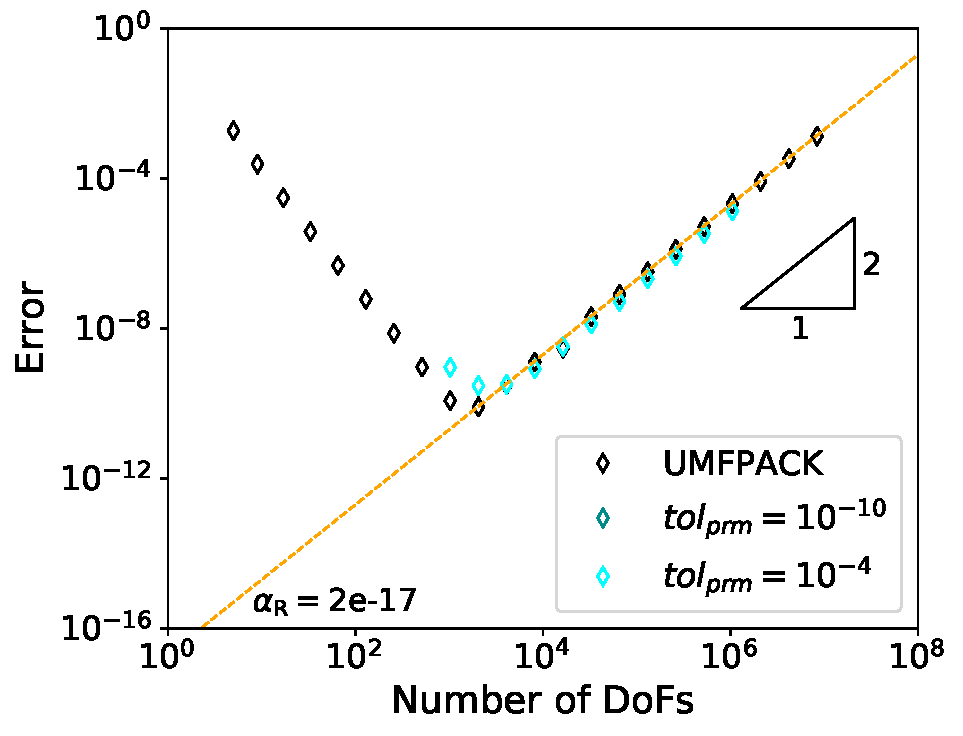
\includegraphics[width=1.0\linewidth]{../2_figure/7_solution_strategy/2_one_degree_for_all_var/1_SM/py_error_comparison_solution_strategy_sm_solu.pdf}
        \caption{$u$}
        \label{py_bench_Pois_SM_error_solution_strategy_solu}
    \end{subfigure}
    \hspace{-0.2cm}
    \begin{subfigure}{5.5cm}
        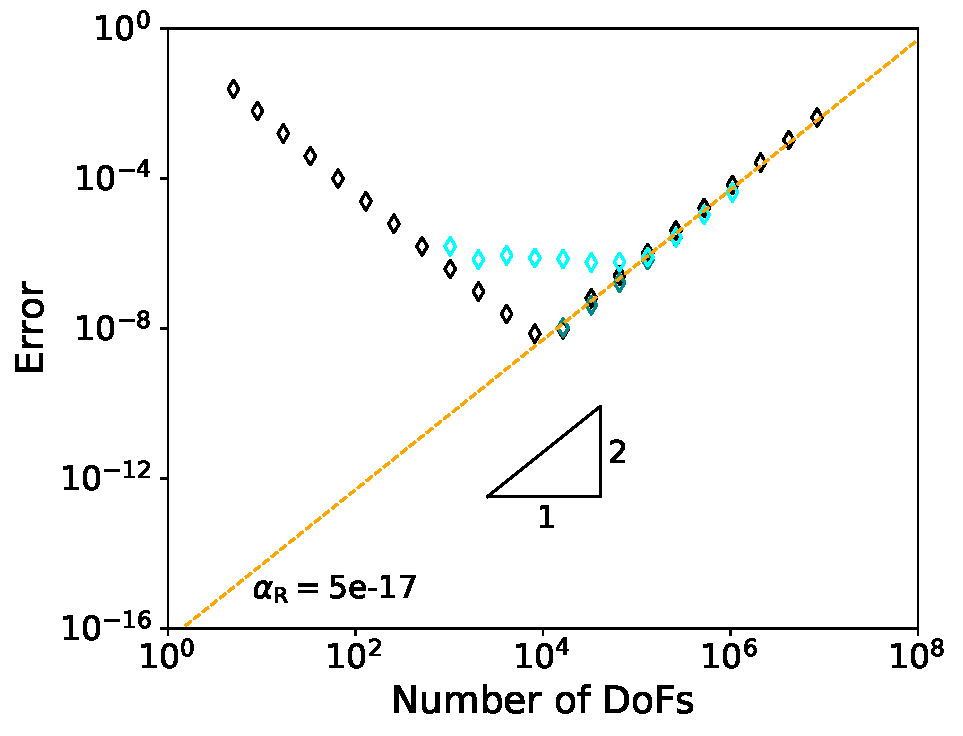
\includegraphics[width=1.0\linewidth]{../2_figure/7_solution_strategy/2_one_degree_for_all_var/1_SM/py_error_comparison_solution_strategy_sm_grad.pdf}
        \caption{$u_x$}
        \label{py_bench_Pois_SM_error_solution_strategy_grad}
    \end{subfigure}
    \hspace{-0.2cm}
    \begin{subfigure}{5.5cm}
        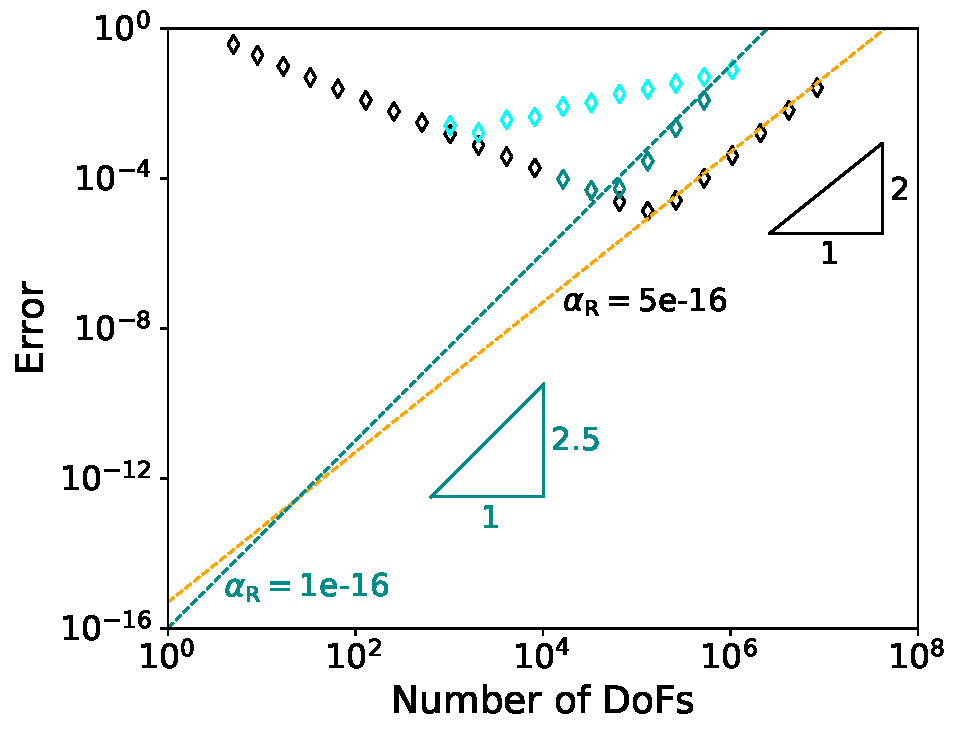
\includegraphics[width=1.0\linewidth]{../2_figure/7_solution_strategy/2_one_degree_for_all_var/1_SM/py_error_comparison_solution_strategy_sm_2ndd.pdf}
        \caption{$u_{xx}$}
        \label{py_bench_Pois_SM_error_solution_strategy_2ndd}
    \end{subfigure}
\caption{Influence of the CG solver on the accuracy using the standard FEM.}
\label{py_bench_Pois_SM_error_solution_strategy}
\end{figure}

When $tol_{prm}$ is adequately small, i.e. $tol_{prm}=10^{-10}$, the round-off error for the solution and the first derivative using the CG solver is the same with that using the UMFPACK solver; the round-off error for the second derivative using the CG solver increases faster than that using the UMFPACK solver.
When $tol_{prm}$ is too large, i.e. $tol_{prm}=10^{-4}$, the error contribution due to the iterative solver dominates both truncation and round-off errors for an intermediate number of DoFs. 

\paragraph{The mixed FEM}

Since the resulting matrix Eq.~(\ref{matrix_equation_mix}) is indefinite, a widely used alternative is to decouple the fully coupled monolithic approach using Schur's complement
\begin{subequations}
 \begin{align}
  B^{\top} M^{-1} B U &= B^{\top} M^{-1} G - H, 	\label{schur_complement_solution} \\
  MV&=G-BU						\label{schur_complement_gradient}
\end{align}						\label{schur_complement_block}%
\end{subequations}
and solve both equations in segregated manner, i.e. Eq. (\ref{schur_complement_solution}) is solved in the first place to obtain $U$, which is then substituted into Eq. (\ref{schur_complement_gradient}) to obtain $V$.

Eq. (\ref{schur_complement_solution}) involves the term $M^{-1} G$ in the right-hand side, which is computed by solving the auxiliary linear system $MY=G$ by using either the UMFPACK or the CG solver. The same options are available for solving Eq. (\ref{schur_complement_gradient}). 

The difficulty in solving Eq. (\ref{schur_complement_solution}) lies in not assembling the Schur complement matrix explicitly since it comprises $M^{-1}$. 
The CG solver only makes use of matrix-vector products of the form $(B^{\top}M^{-1}B)W$, which can be computed by the following three-step algorithm: $X=BW$, $MY=X$ and $Z=B^{\top}Y$. As before, the linear system $MY=X$ can be solved by the UMFPACK or the CG solver.

We first investigate the influence of $tol_{prm}$ of the CG solver on the accuracy of the solutions when the left-hand side is $B^{\top}M^{-1}B$. In this case, the UMFPACK solver is used to solve the matrix equations when the left-hand side is $M$.  
For $tol_{prm}$ being $10^{-16}$ and $10^{-10}$, the results are shown in Fig. \ref{py_bench_Pois_MM_error_solution_strategy_schur_variant_other_UMF}, in comparison with that obtained from solving the monolithic Eq. (\ref{matrix_equation_mix}) directly using the UMFPACK solver.
It shows that, for the problem at hand, the monolithic solution approach yields by far the most accurate solution and derivative values. The round-off error for $v_{x}$ increases fastest using the Schur complement approach even though $tol_{prm}$ is sufficiently small, i.e. $tol_{prm}=10^{-16}$, which makes the highest attainable accuracy much lower.
When $tol_{prm}$ is less strict, i.e. $tol_{prm}=10^{-10}$, the iteration error dominates the total error instead of the round-off error.

\begin{figure}[!ht]
    \begin{subfigure}{5.5cm}
        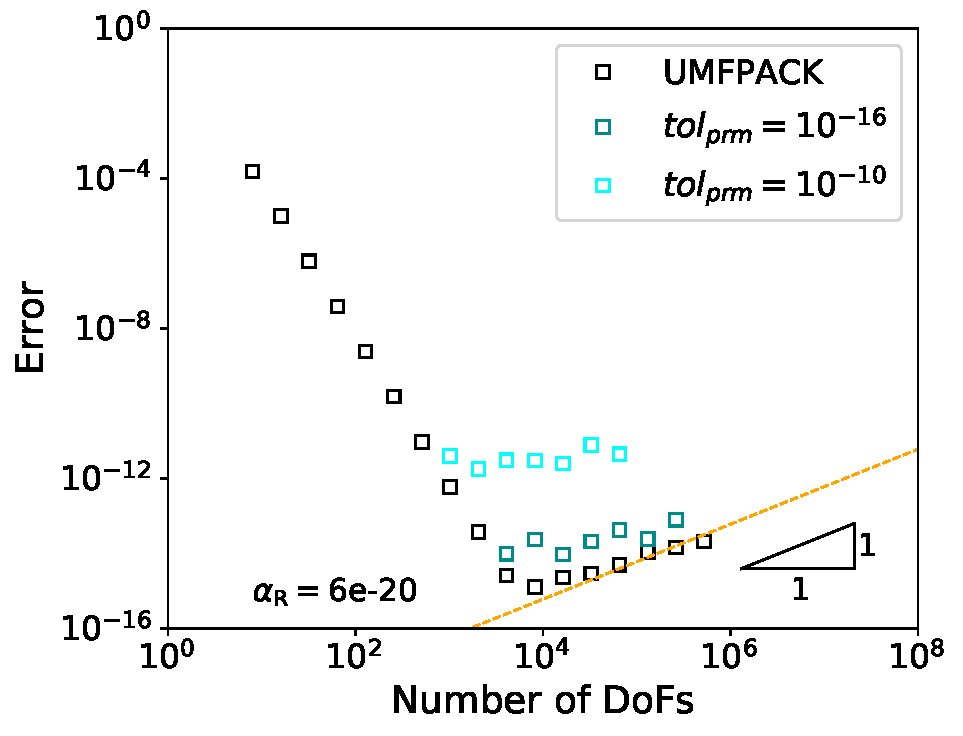
\includegraphics[width=1.0\linewidth]{../2_figure/7_solution_strategy/2_one_degree_for_all_var/2_MM/1_1_Schur_variant_M_UMF/py_error_comparison_solution_strategy_mm_Schur_var_M_umf_solu.pdf}
        \caption{$u$}
        \label{py_bench_Pois_MM_error_solution_strategy_schur_variant_other_UMF_solu}
    \end{subfigure}
    \hspace{-0.2cm}
    \begin{subfigure}{5.5cm}
        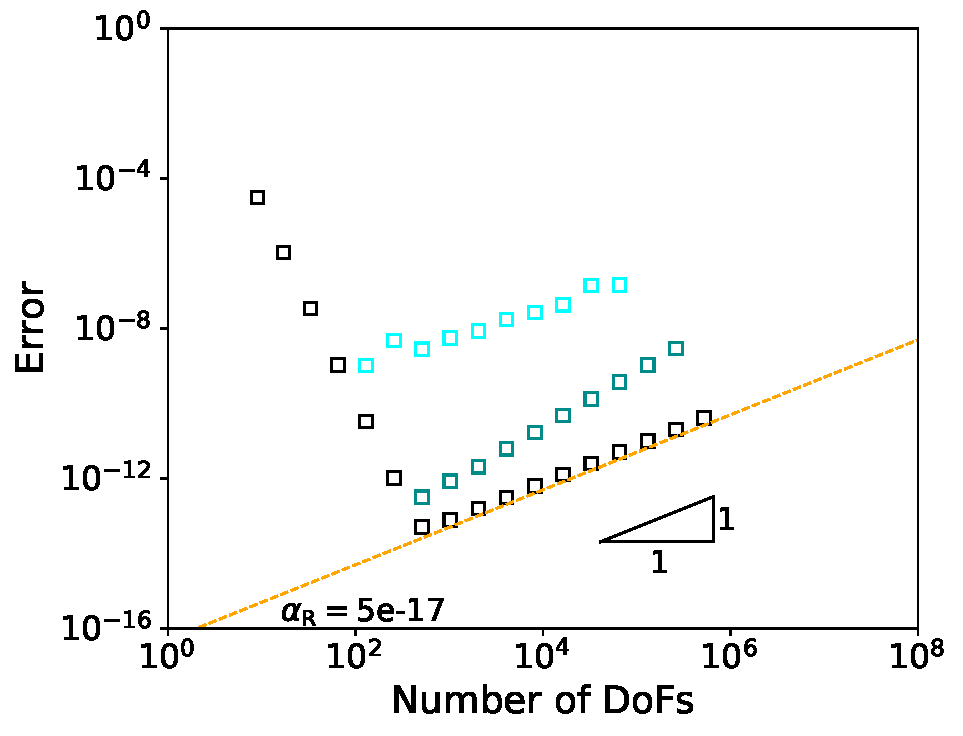
\includegraphics[width=1.0\linewidth]{../2_figure/7_solution_strategy/2_one_degree_for_all_var/2_MM/1_1_Schur_variant_M_UMF/py_error_comparison_solution_strategy_mm_Schur_var_M_umf_grad.pdf}
        \caption{$v$}
        \label{py_bench_Pois_MM_error_solution_strategy_schur_variant_other_UMF_grad}
    \end{subfigure}
    \hspace{-0.2cm}
    \begin{subfigure}{5.5cm}
        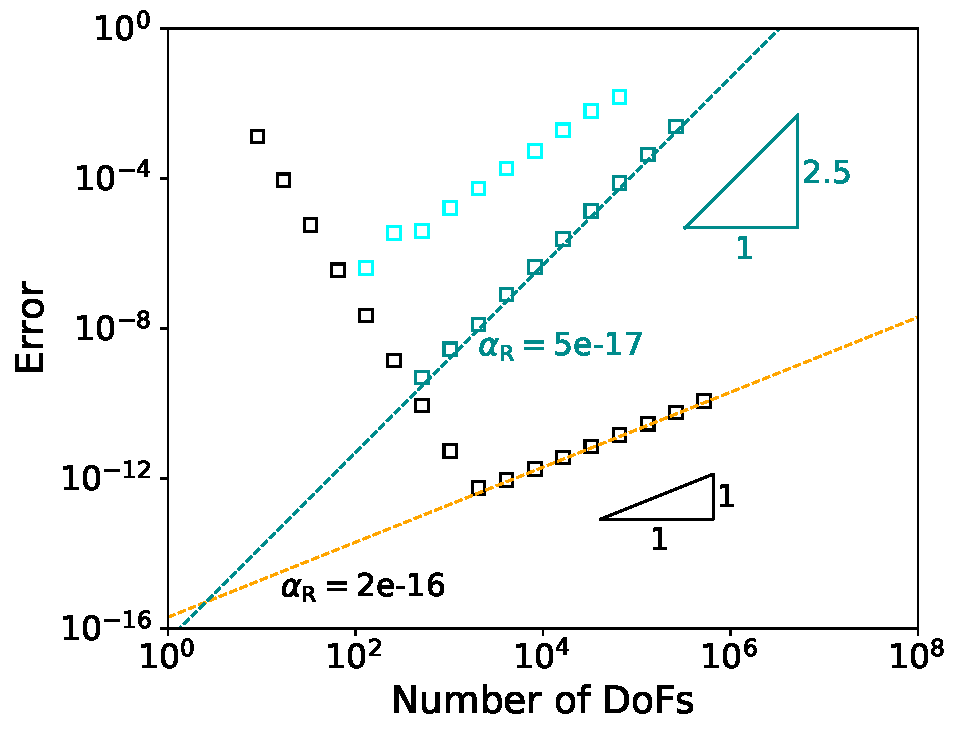
\includegraphics[width=1.0\linewidth]{../2_figure/7_solution_strategy/2_one_degree_for_all_var/2_MM/1_1_Schur_variant_M_UMF/py_error_comparison_solution_strategy_mm_Schur_var_M_umf_2ndd.pdf}
        \caption{$v_x$}
        \label{py_bench_Pois_MM_error_solution_strategy_schur_variant_other_UMF_2ndd}
    \end{subfigure}
\caption{Influence of the CG solver on the accuracy when the left-hand side is the Schur complement using the mixed FEM.}
\label{py_bench_Pois_MM_error_solution_strategy_schur_variant_other_UMF}
\end{figure}

Next, we investigate the influence of $tol_{prm}$ of the CG solver when the left-hand side is $M$. In this case, the CG solver with $tol_{prm}$ being $10^{-16}$ is used to solve the matrix equation with the left-hand side being $B^{\top}M^{-1}B$. For $tol_{prm}$ being $10^{-16}$ and $10^{-10}$, the results are shown in Fig.~\ref{py_bench_Pois_MM_error_solution_strategy_schur_1em16_M_variant}, in comparison with that obtained from solving the monolithic Eq. (\ref{matrix_equation_mix}) directly using the UMFPACK solver.
It also shows that, when the tolerance is less strict, i.e. $tol_{prm}=10^{-10}$, the iteration error dominates the total error before the round-off error.

\begin{figure}[!ht]
    \begin{subfigure}{5.5cm}
        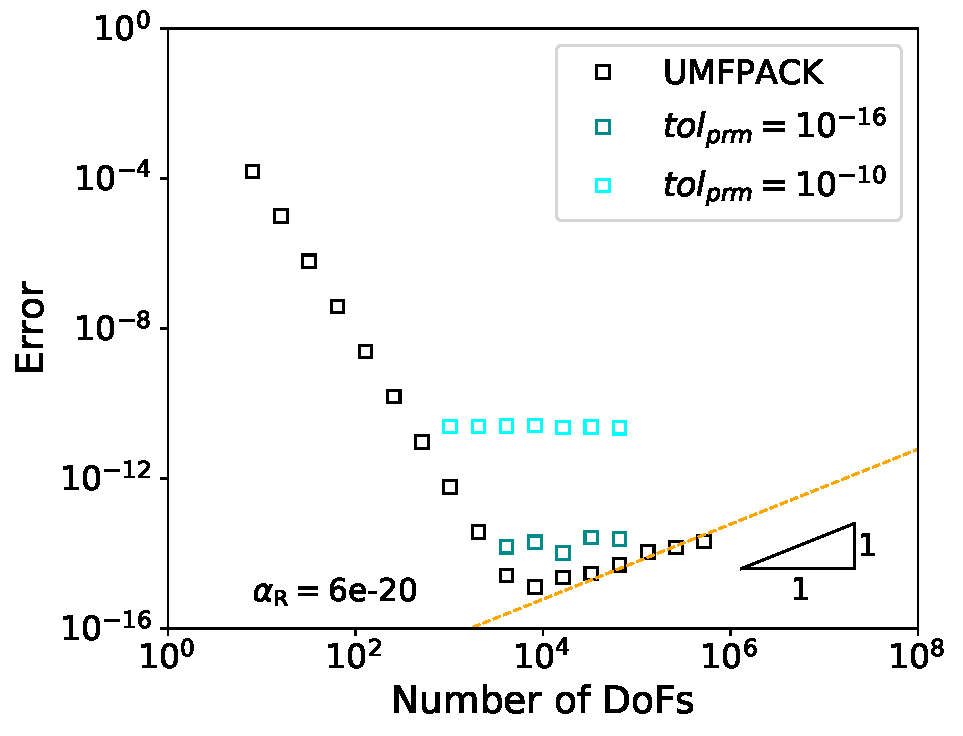
\includegraphics[width=1.0\linewidth]{../2_figure/7_solution_strategy/2_one_degree_for_all_var/2_MM/1_1_Schur_variant_M_UMF/py_error_comparison_solution_strategy_mm_M_var_Schur_1em16_solu.pdf}
        \caption{$u$}
        \label{py_bench_Pois_MM_error_solution_strategy_schur_1em16_M_variant_solu}
    \end{subfigure}
    \hspace{-0.2cm}
    \begin{subfigure}{5.5cm}
        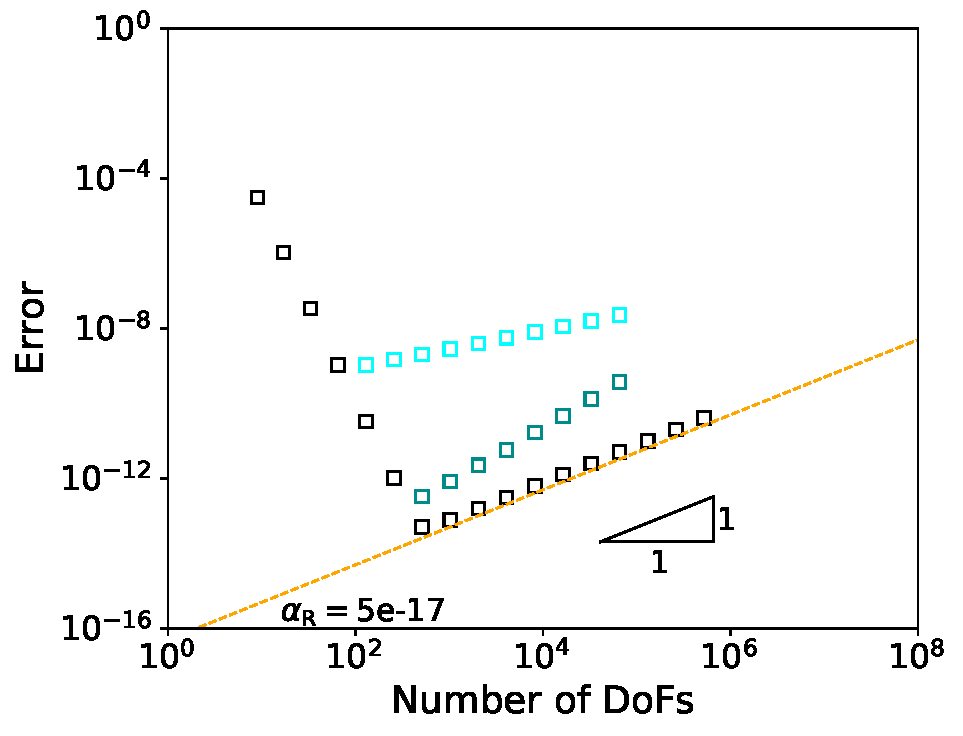
\includegraphics[width=1.0\linewidth]{../2_figure/7_solution_strategy/2_one_degree_for_all_var/2_MM/1_1_Schur_variant_M_UMF/py_error_comparison_solution_strategy_mm_M_var_Schur_1em16_grad.pdf}
        \caption{$v$}
        \label{py_bench_Pois_MM_error_solution_strategy_schur_1em16_M_variant_grad}
    \end{subfigure}
    \hspace{-0.2cm}
    \begin{subfigure}{5.5cm}
        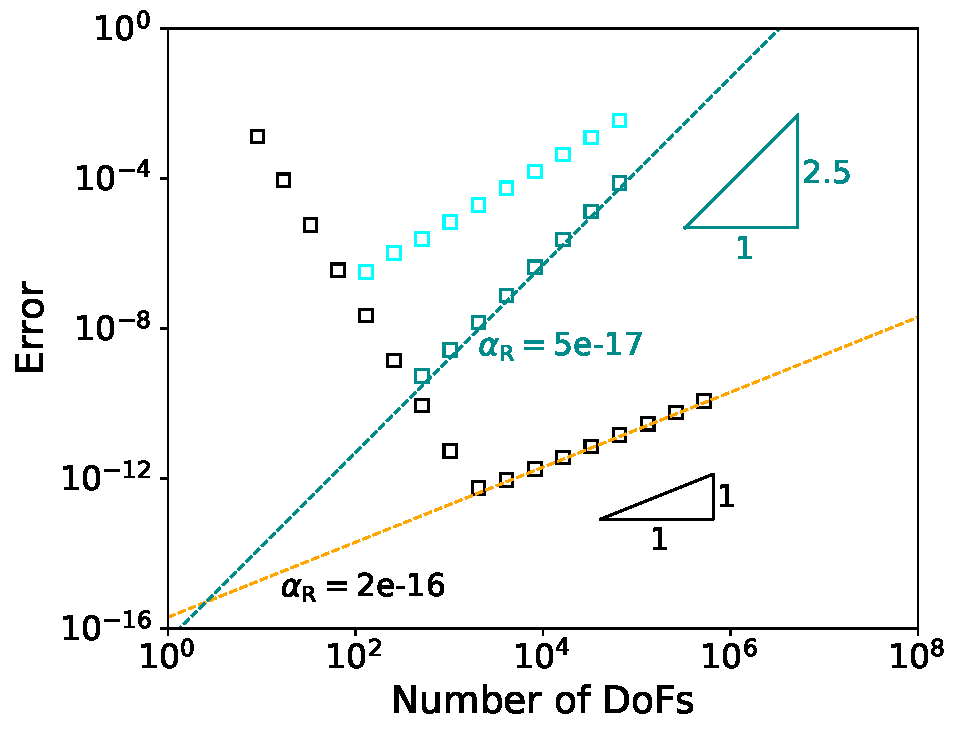
\includegraphics[width=1.0\linewidth]{../2_figure/7_solution_strategy/2_one_degree_for_all_var/2_MM/1_1_Schur_variant_M_UMF/py_error_comparison_solution_strategy_mm_M_var_Schur_1em16_2ndd.pdf}
        \caption{$v_x$}
        \label{py_bench_Pois_MM_error_solution_strategy_schur_1em16_M_variant_2ndd}
    \end{subfigure}
\caption{Influence of the CG solver on the accuracy when the left-hand side is $M$ using the mixed FEM.}
\label{py_bench_Pois_MM_error_solution_strategy_schur_1em16_M_variant}
\end{figure}

In summary, in comparison with the UMFPACK solver, the CG solver gives the same accuracy for $u$ and $u_{x}$ but less accuracy for $u_{xx}$ using the standard FEM, and gives smaller accuracy for all the three variables using the mixed FEM when $tol_{prm}$ is strict enough; the CG solver introduces iteration errors for both the standard FEM and the mixed FEM when $tol_{prm}$ is less strict. Thereby, we continue with the UMFPACK solver in our algorithm to obtain higher accuracy.


\subsubsection{Boundary condition}	\label{section_sensitivity_BC}

In this section, two aspects of the influence of the boundary conditions on the round-off error are investigated: first the method of implementing the Dirichlet boundary conditions, and secondly types of boundary conditions. 

For the first aspect, using Weak form 2 for $\rho=50$ and $10^6$, the errors are depicted in Fig.~\ref{py_bench_Pois_SM_error_boundary_weak}, in comparison with that using Weak form 1. As can be seen, both the weak imposition and the strong imposition of the Dirichlet boundary condition yield the same trend line for the round-off error for the solution and its derivatives, and the magnitude of the penalty parameter in the weak imposition makes no difference. In addition, small penalty parameters might lead to larger truncation errors for $u$, but the difference diminishes when the penalty parameter is large enough.

\begin{figure}[!ht]
    \begin{subfigure}{5.5cm}
        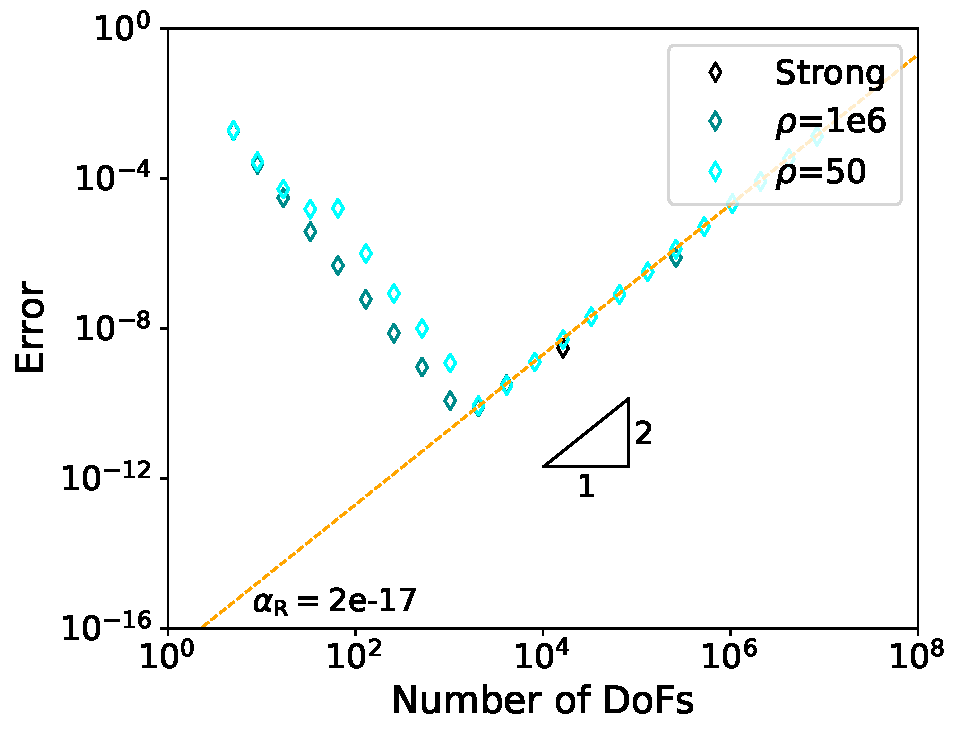
\includegraphics[width=1.0\linewidth]{../2_figure/6_boundary_condition/1_weak_imposition/py_bench_Pois_SM_error_boundary_weak_solu.pdf}
        \caption{$u$}
        \label{py_bench_Pois_SM_error_boundary_weak_solu}
    \end{subfigure}
    \hspace{-0.2cm}
    \begin{subfigure}{5.5cm}
        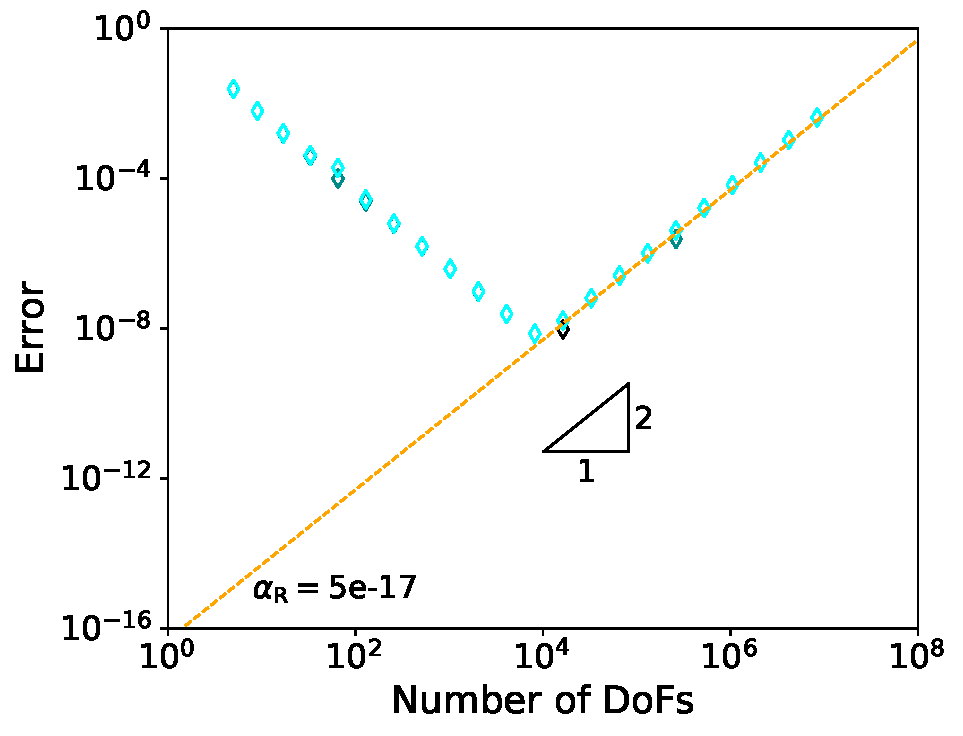
\includegraphics[width=1.0\linewidth]{../2_figure/6_boundary_condition/1_weak_imposition/py_bench_Pois_SM_error_boundary_weak_grad.pdf}
        \caption{$u_x$}
        \label{py_bench_Pois_SM_error_boundary_weak_grad}
    \end{subfigure}
    \hspace{-0.2cm}
    \begin{subfigure}{5.5cm}
        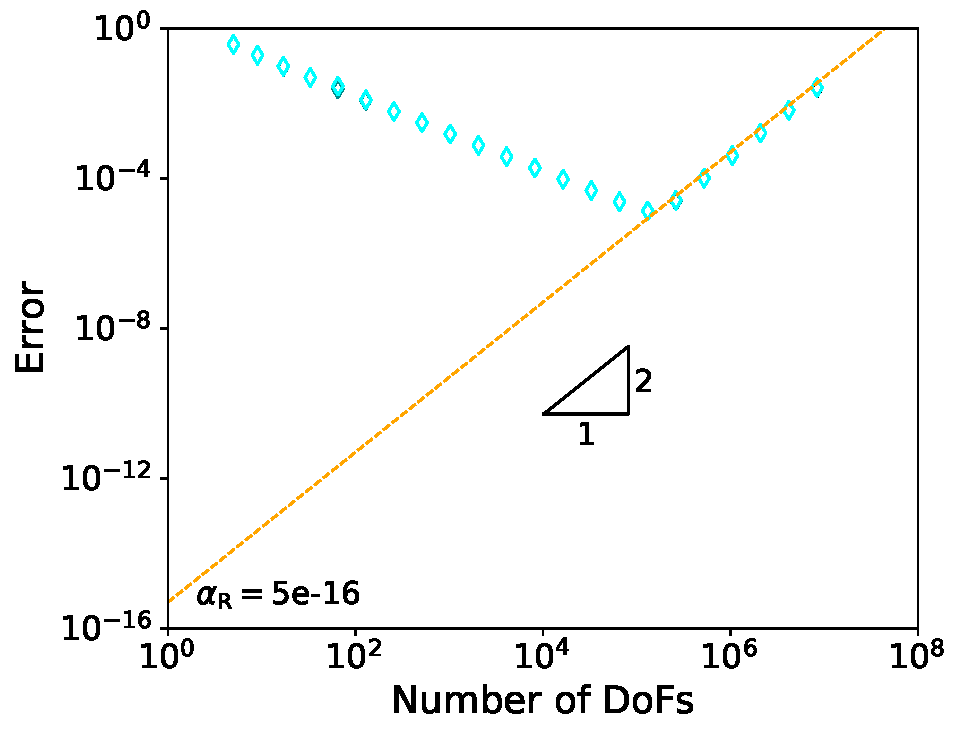
\includegraphics[width=1.0\linewidth]{../2_figure/6_boundary_condition/1_weak_imposition/py_bench_Pois_SM_error_boundary_weak_2ndd.pdf}
        \caption{$u_{xx}$}
        \label{py_bench_Pois_SM_error_boundary_weak_2ndd}
    \end{subfigure}
\caption{Influence of the weak imposition of the Dirichlet boundary condition on the accuracy.}
\label{py_bench_Pois_SM_error_boundary_weak}
\end{figure}

To construct the problem for the second aspect, the Dirichlet boundary condition at the left boundary ($x=0$) is kept while the Dirichlet boundary condition at the right boundary ($x=1$) is replaced by the Neumann boundary condition $u_x (1) = -e^{-1/4}$, leading to the same solution and derivative profiles. 


% \newpage
\paragraph{The standard FEM}
Using the standard FEM, the offsets $\alpha_{\rm R}$ for the two types of boundary conditions are depicted in Fig.~\ref{boundary_type_benchmark_Poisson_std}. 
For the Dirichlet/Neumann boundary condition, the offsets $\alpha_{\rm R}$ for $u$ and $u_x$ are slightly larger than that for the Dirichlet/Dirichlet boundary condition by a factor of 3.5 and 2, respectively. The offsets $\alpha_{\rm R}$ for $u_{xx}$ are identical for the two types of boundary conditions.

\paragraph{The mixed FEM}
Using the mixed FEM, the offsets $\alpha_{\rm R}$ for the two types of boundary conditions are depicted in Fig.~\ref{boundary_type_benchmark_Poisson_mix}.
As can be seen, the type of boundary conditions plays a more important role for $\alpha_{\rm R}$ for the solution than $\alpha_{\rm R}$ for other variables.


\begin{figure}[!ht]
\hspace{2.2cm}
% \centering
\begin{subfigure}[b]{0.4\textwidth}
\scalebox{0.9}{
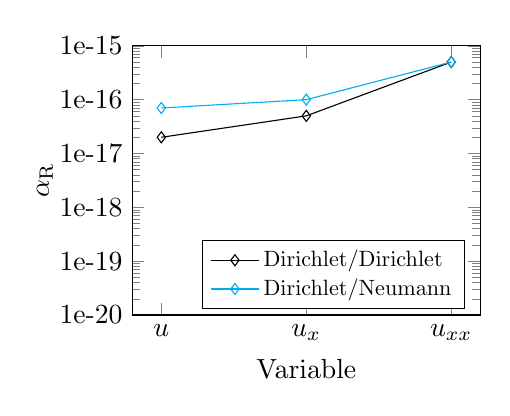
\begin{tikzpicture} 
\begin{axis}
[
    ymode=log,    
    ymin=1e-20,
    ymax=1e-15,
    ytick={1e-20,1e-19,1e-18,1e-17,1e-16,1e-15},
    yticklabels={1e-20,1e-19,1e-18,1e-17,1e-16,1e-15},      
    legend style={nodes={scale=0.8},at={(0.2,0.15)},anchor=west},
    legend cell align={left},
    height=5cm,
    width=6cm,
    ylabel={$\alpha_{\rm R}$},
	ylabel style={at={(-0.2,0.5)}},    
    xtick={0,1,2},
    xticklabels={$u$,$u_x$, $u_{xx}$},
    xlabel={Variable},
    xlabel style={at={(0.5,-0.13)}}  
]
\addplot[black,mark=diamond,mark options={color=black,fill=black}] coordinates {(0,2.0e-17) (1,5.0e-17) (2,5.0e-16)};
\addplot[cyan,mark=diamond,mark options={color=cyan,fill=cyan}] coordinates {(0,7.0e-17) (1,1.0e-16) (2,5.0e-16)};
\legend{Dirichlet/Dirichlet, Dirichlet/Neumann};
\end{axis}
\end{tikzpicture}
}
\caption{The standard FEM}
\label{boundary_type_benchmark_Poisson_std}
\end{subfigure}
\hspace{-1.0cm}
\begin{subfigure}[b]{0.4\textwidth}
\scalebox{0.9}{
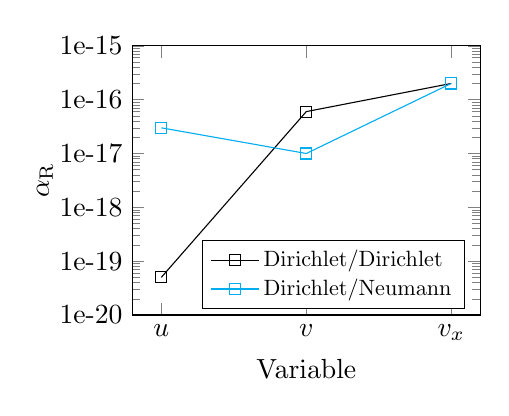
\begin{tikzpicture} 
\begin{axis}
[
    ymode=log,    
    ymin=1e-20,
    ymax=1e-15,
    ytick={1e-20,1e-19,1e-18,1e-17,1e-16,1e-15},
    yticklabels={1e-20,1e-19,1e-18,1e-17,1e-16,1e-15},        
    legend style={nodes={scale=0.8},at={(0.2,0.15)},anchor=west},
    legend cell align={left},
    height=5cm,
    width=6cm,
    ylabel={$\alpha_{\rm R}$},
	ylabel style={at={(-0.2,0.5)}},    
    xtick={0,1,2},
    xticklabels={$u$,$v$, $v_x$},
    xlabel={Variable},
    xlabel style={at={(0.5,-0.13)}}    
]
\addplot[black,mark=square,mark options={color=black,fill=black}] coordinates {(0, 5.0e-20) (1, 6.0e-17) (2, 2.0e-16)};
\addplot[cyan,mark=square,mark options={color=cyan,fill=cyan}] coordinates {(0, 3.0e-17) (1, 1.0e-17) (2, 2.0e-16)};
\legend{Dirichlet/Dirichlet, Dirichlet/Neumann};
\end{axis}
\end{tikzpicture}
}
\caption{The mixed FEM}
\label{boundary_type_benchmark_Poisson_mix}
\end{subfigure}
\caption{Comparison of the errors for imposing Dirichlet/Dirichlet and Dirichlet/Neumann boundary conditions.}
\label{boundary_type_benchmark_Poisson}
\end{figure}

In summary, $\alpha_{\rm R}$ are relatively independent of the variations in the type of boundary conditions and the method Dirichlet boundary conditions are implemented, which is an important prerequisite for our a posteriori refinement strategy to be applicable for a wide range of problems. However, since the asymptotic behaviour of the truncation error is essential in our algorithm, we continue with the strong imposition of the Dirichlet boundary condition.

In Sections \ref{section_general_poisson} -- \ref{section_d_and_r}, where the influences of $u(x)$, $d(x)$ and $r(x)$ are investigated, we only consider the Dirichlet boundary conditions, and still use $P_2$ elements for the standard FEM and $P_4/P_3^{\rm disc}$ elements for the mixed FEM.


\subsection{General Poisson equation}	    \label{section_general_poisson}

In this section, we will again consider the Poisson equation, but now focus on the influence of the order of magnitude of the solution and right-hand side on $\alpha_{\rm R}$.
To cover a wide range of scenarios, we choose the cases shown in Table \ref{scaling_cases_Poisson}. 
Each case contains a coefficient $c_i,~i=1,2, \ldots , 5$, which is varied over several orders of magnitude so that the $L_2$ norm of the solution, denoted by $\|u\|_2$, and the $L_2$ norm of the right-hand side, denoted by $\|f\|_2$, extend over a wide range of magnitudes. Fig.~\ref{l2_norm_u_f} gives an overview of the distribution of $\|u\|_2$ and $\|f\|_2$ for Cases 1--4.

\begin{table}[!ht]
\small
\centering
\caption [w]{Setting of the Poisson equation with different right-hand sides.} 
\label{scaling_cases_Poisson}
 \begin{tabular}{c | c | c | c | c} \hline      
\multirow{2}{*}{Case} & \multirow{2}{*}{$f(x)$}  & \multicolumn{2}{c|}{Boundary conditions} & \multirow{2}{*}{$u(x)$} \\
\cline{3-4}
& & $u(0)$ & $u(1)$ & \\ \hline
{1} & {$\sin (2 \pi c_1x)$} & {0}& ${(2 \pi c_1)}^{-2} \sin (2 \pi c_1)$ & ${(2 \pi c_1)}^{-2} \sin (2 \pi c_1x)$\\ \hline
2 & $\makecell{-e^{-{c_2}{(x-1/2)^2}} \cdot \\ \left({4{c_2}^2(x-1/2)^2 -2c_2} \right)}$ & $e^{-c_2/4}$ & $e^{-c_2/4}$ & $e^{-{c_2}{{(x-1/2)^2}}}$ \\ \hline
3 & $\sin (2 \pi c_3 x) +1$ & $0$ & ${(2 \pi c_3)}^{-2}\sin (2 \pi c_3)-\frac{1}{2}$ & ${(2 \pi c_3)}^{-2}\sin (2 \pi c_3 x)-\frac{x^2}{2}$ \\ \hline
4 & $(2 \pi c_4) \sin (2 \pi c_4 x)$ & $0$ & ${(2 \pi c_4)}^{-1} \sin (2 \pi c_4)$ & ${(2 \pi c_4)}^{-1} \sin (2 \pi c_4x)$ \\ \hline
5 & $0$ & $0$ & ${c_5}^{-1}$ & ${c_5}^{-1} x$ \\ \hline
\end{tabular}
\end{table}


\begin{figure}[!ht]
\centering
    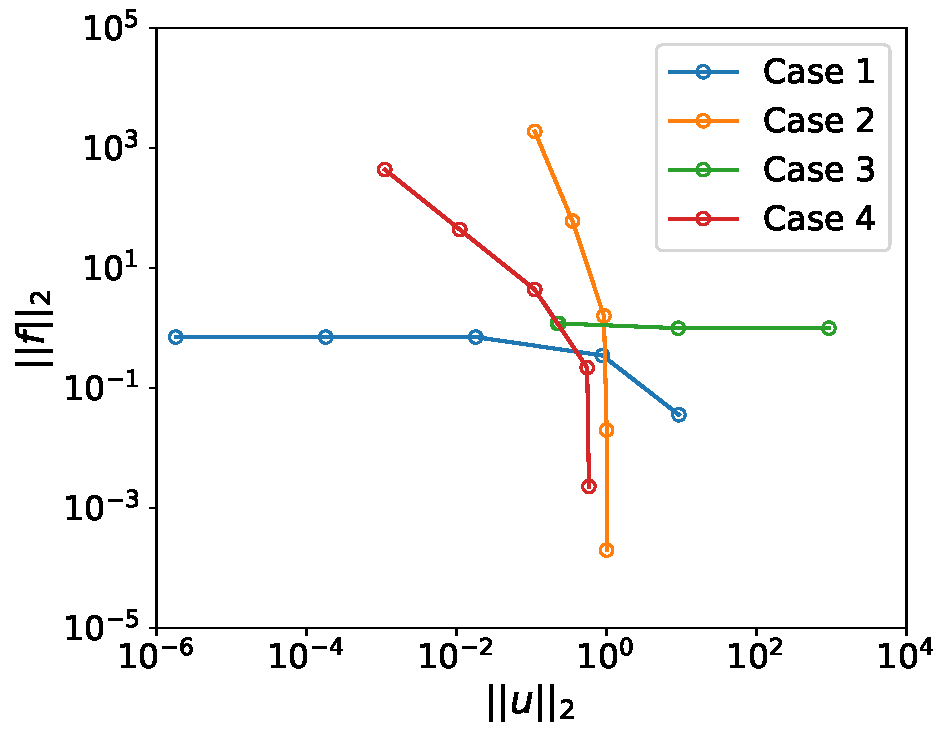
\includegraphics[width=0.42\linewidth]{../2_figure/2_l2_norm_u_f/l2_norm_u_f.pdf}
    \caption{Distribution of $\|u\|_2$ and $\|f\|_2$ of the Poisson equations in Table~\ref{scaling_cases_Poisson}.}
    \label{l2_norm_u_f}
\end{figure}

For these Poisson problems, the error basically evolves according to that shown in Fig.~\ref{error_evolution_one_p}. To summarize, $\beta_{\rm R}$ is 2 using the standard FEM and 1 using the mixed FEM. $\alpha_{\rm R}$ against $\|u\|_2$ is shown in Fig. \ref{py_offset_summary_Pois_sm} for the standard FEM; $\alpha_{\rm R}$ against $\|u\|_2$ or $\|v\|_2$, depending on the dependent variable of interest, is shown in Fig. \ref{py_offset_summary_Pois_mm} for the mixed FEM.

For all the variables using both the standard FEM and the mixed FEM, the distribution of $\alpha_{\rm R}$ can be approximated by a straight line. This implies that $\alpha_{\rm R}$ has a power-law relation with the horizontal coordinate. The power term, represented by the slope of the line, is 1 for all the relations; the constant term, represented by the intercept of the line, is denoted in the figure. The latter reads 2e-17, 5e-17 and 5e-16 for $u$, $u_x$ and $u_{xx}$, respectively, using the standard FEM, and 1e-18, 1e-16 and 5e-16 for $u$, $v$ and $v_x$, respectively, using the mixed FEM. Note that, the intercept is the value of $\alpha_{\rm R}$ when the horizontal coordinate is 1. Therefore, $\alpha_{\rm R}$ has a linear relation with the $L_2$ norm of the dependent variable. We express $\alpha_{\rm R}$ as the product of a constant and the magnitude of $\|u\|_2$ or $\|v\|_2$ that is shown in Table~\ref{relation_alpha_R_l2_norm}.

\begin{figure}[!ht]
	\centering
    \begin{subfigure}{6.0cm}
        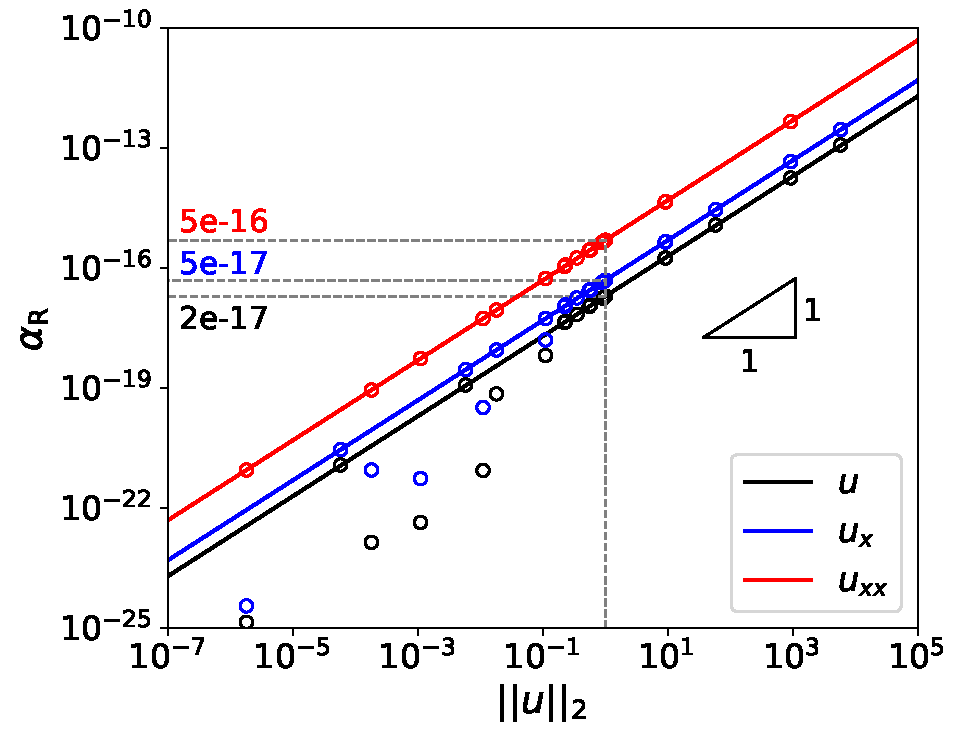
\includegraphics[width=1.0\linewidth]{../2_figure/4_offset_summary/py_offset_summary_Pois_sm.pdf}
        \caption{The standard FEM}
        \label{py_offset_summary_Pois_sm}
    \end{subfigure}
    \hspace{-0.2cm}
    \begin{subfigure}{6.0cm}
        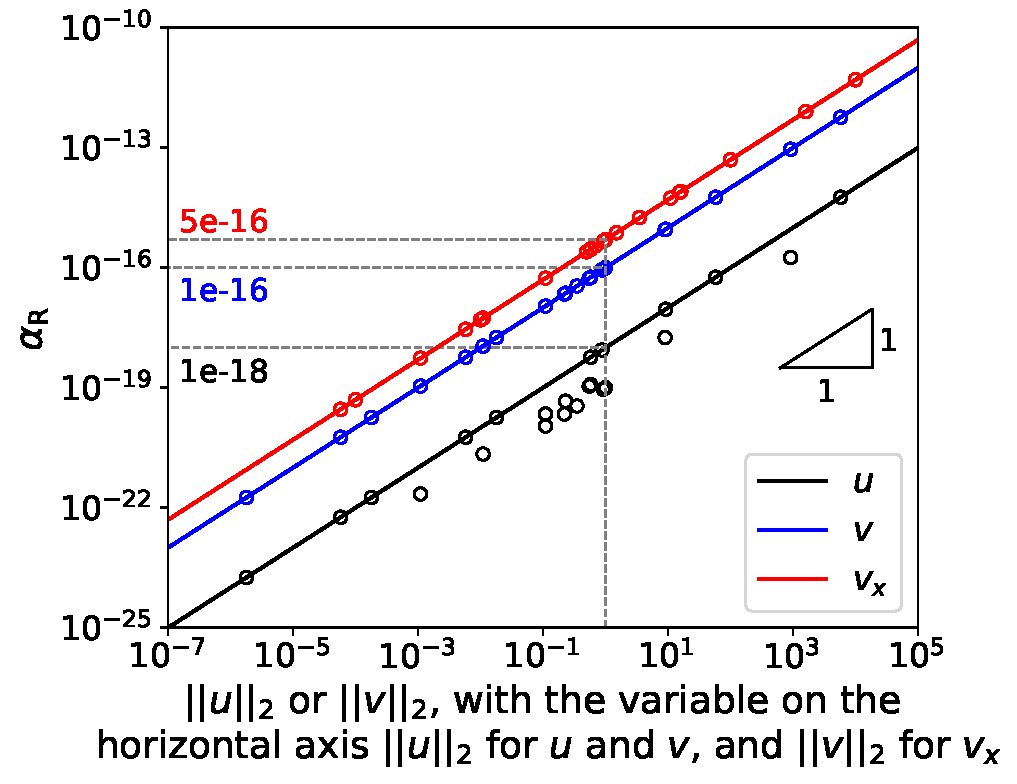
\includegraphics[width=1.0\linewidth]{../2_figure/4_offset_summary/py_offset_summary_Pois_mm.pdf}
        \caption{The mixed FEM}
        \label{py_offset_summary_Pois_mm}
    \end{subfigure}
\caption{$\alpha_{\rm R}$ for the influence of $u(x)$.}
\label{py_offset_summary_Pois}
\end{figure}

\begin{table}[!ht]
\small
\captionof{table}{$\alpha_{\rm R}$ in terms of the product of a constant and the $L_2$ norm $\|u\|_2$ or $\|v\|_2$, dependent on the specific dependent variable, for one-dimensional Poisson equations.}
\hspace{3.5cm}
\begin{subtable}{0.4\textwidth}
\caption{The standard FEM}
\label{relation_alpha_R_l2_norm_std}
\begin{tabular}{c | l c}
\hline
Variable & \multicolumn{2}{c}{$\alpha_{\rm R}$} \\ \hline
$u$ & 2e-17 & \multirow{3}{*}{$\Bigg\}\times \|u\|_2$} \\ \cline{1-2}
$u_x$ & 5e-17 & \\ \cline{1-2}
$u_{xx}$ & 5e-16 & \\ \hline
\end{tabular}
\end{subtable}
\hspace{-2cm}
\begin{subtable}{.4\textwidth}
\caption{The mixed FEM}
\label{relation_alpha_R_l2_norm_mix}
\begin{tabular}{c | l c}
\hline
Variable & \multicolumn{2}{c}{$\alpha_{\rm R}$} \\ \hline
$u$ & 1e-18 & \multirow{2}{*}{$\bigg\}\times\|u\|_2$} \\ \cline{1-2} 
$v$ & 1e-16 &  \\ \hline
$v_x$ & 5e-16 & $\times \|v\|_2$ \\ \hline
\end{tabular}
\end{subtable}
\label{relation_alpha_R_l2_norm}
\end{table}

\subsection{General diffusion and Helmholtz equation}	\label{section_d_and_r}

The coefficient $d(x)$ is taken from Table~\ref{d_diffusion_equations} for the diffusion equations, and $d(x)=1$ is taken for the Helmholtz equations, with $r(x)$ taken from Table~\ref{r_Helmholtz_equations}. The analytical solution $u$ is the same as the benchmark Poisson equation, of which $\|u\|_2=0.92$ and $\|v\|_2=0.5$. 

\begin{table}[!ht]
\centering
\caption [w]{Various $d(x)$ for the diffusion equations.} 
\label{d_diffusion_equations}
 \begin{tabular}{c | c | c | c | c | c} \hline
Case &$d(x)$ & $\|d\|_2$ & Case &$d(x)$ & $\|d\|_2$ \\ \hline
1 & 0.01 & 0.01 & 7 & $1+\sin(10x)$ & 1.14 \\ \hline
2 & 0.1 & 0.1 & 8 & $1+\sin(100x)$ & 1.06 \\ \hline
3 & 1 & 1 & 9 & $1+x$ & 1.5 \\ \hline
4 & 10 & 10 & 10 & $1+10x$ & 6.7 \\ \hline
5 & 100 & 100 & 11& $1+100x$ & 58.6 \\ \hline
6 & $1+\sin(x)$ & 1.23 & \multicolumn{3}{c}{} \\ \hline
\end{tabular}
\end{table}

\begin{table}[!ht]
\centering
\caption [w]{Various $r(x)$ for the Helmholtz equations.} 
\label{r_Helmholtz_equations}
 \begin{tabular}{c | c | c} \hline
Case & $r(x)$ & $\|r\|_2$ \\ \hline
1 & 0.01 & 0.01 \\ \hline
2 & 0.1 & 0.1 \\ \hline 
3 & 1 & 1 \\ \hline 
4 & 10 & 10 \\ \hline 
5 & 100 & 100 \\ \hline
\end{tabular}
\end{table}

Again the errors show the same behaviour as that shown in Fig.~\ref{error_evolution_one_p}. The coefficient $\beta_{\rm R}$ is 2 using the standard FEM and 1 using the mixed FEM. 

The parameter $\alpha_{\rm R}$ against $\|d\|_2$ is shown in Fig.~\ref{py_offset_summary_diff} for the diffusion equations. Using the standard FEM, $\alpha_{\rm R}$ is independent of $\|d\|_2$ for $u$, $u_x$ and $u_{xx}$, with the upper bound reading 2e-17, 5e-17 and 1e-15, respectively. Using the mixed FEM, $\alpha_{\rm R}$ is independent of $\|d\|_2$ for $u$, but is linearly dependent on $\|d\|_2$ for both $v$ and $v_x$. The upper bound for $u$ reads 5e-17; the intercept for $v$ and $v_x$ reads 2e-16 and 5e-16, respectively.
The parameter $\alpha_{\rm R}$ against $\|r\|_2$ is shown in Fig.~\ref{py_offset_summary_Helm} for the Helmholtz equations.
Visibly, $\alpha_{\rm R}$ is independent of $\|r\|_2$ using both the standard FEM and the mixed FEM. Using the standard FEM, $\alpha_{\rm R}$ reads 2e-17, 5e-17 and 2e-16 for $u$, $u_x$ and $u_{xx}$, respectively; using the mixed FEM, $\alpha_{\rm R}$ reads 1e-19, 1e-16 and 2e-16 for $u$, $v$ and $v_x$, respectively.

\begin{figure}[!ht]
	\centering
    \begin{subfigure}{6.0cm}
        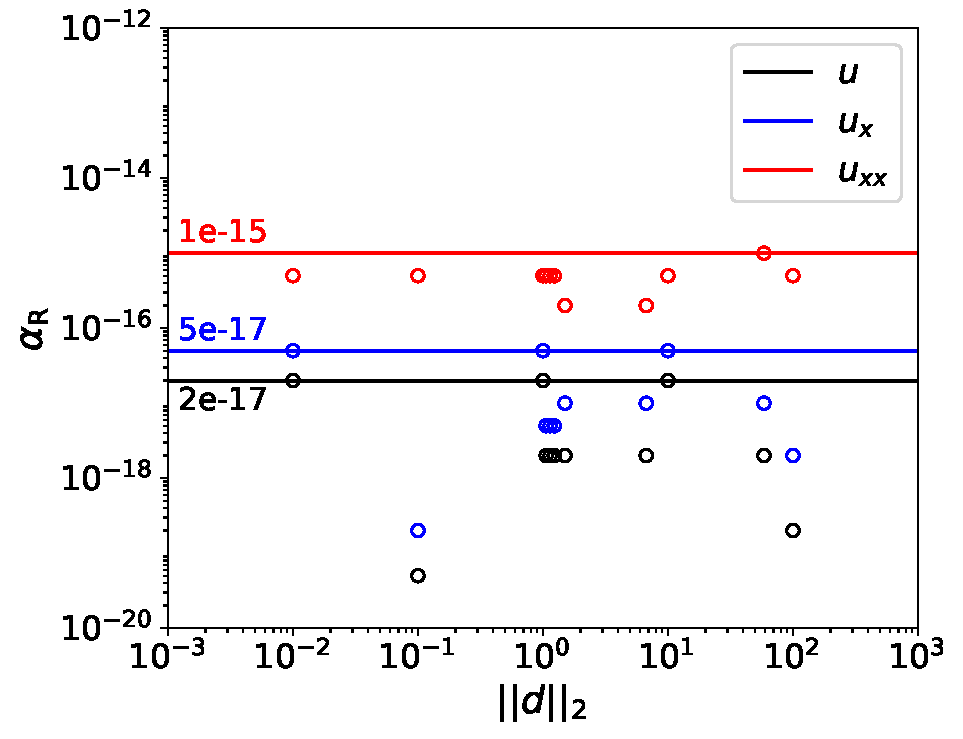
\includegraphics[width=1.0\linewidth]{../2_figure/4_offset_summary/py_offset_summary_diff_sm.pdf}
        \caption{The standard FEM}
        \label{py_offset_summary_diff_sm}
    \end{subfigure}
    \hspace{-0.2cm}
    \begin{subfigure}{6.0cm}
        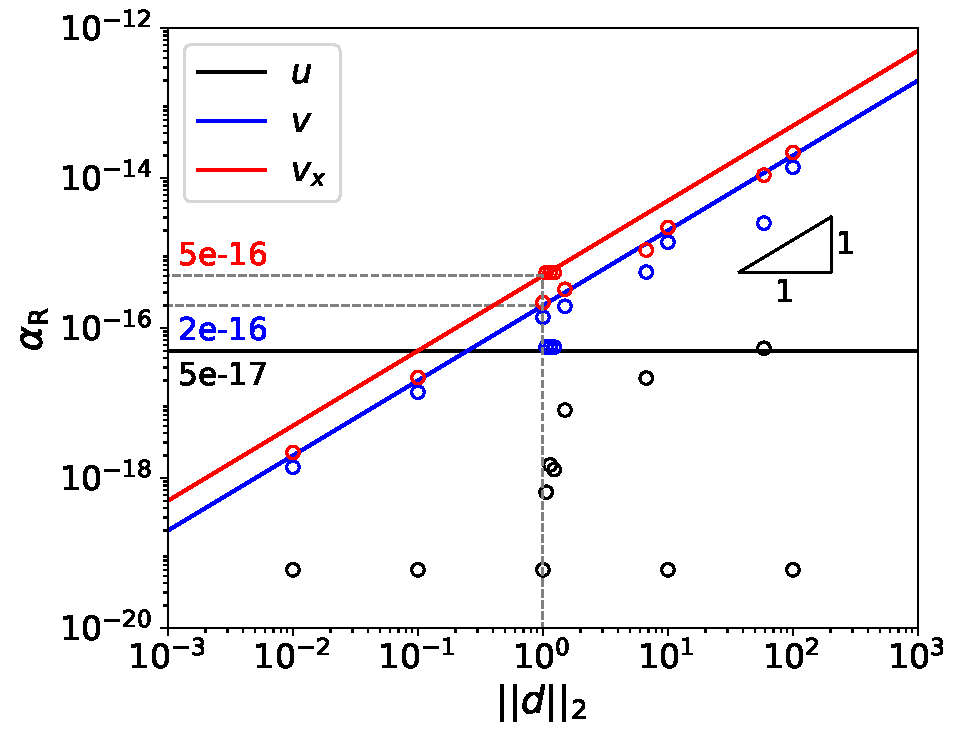
\includegraphics[width=1.0\linewidth]{../2_figure/4_offset_summary/py_offset_summary_diff_mm.pdf}
        \caption{The mixed FEM}
        \label{py_offset_summary_diff_mm}
    \end{subfigure}
\caption{$\alpha_{\rm R}$ for the general diffusion equations.}
\label{py_offset_summary_diff}
\end{figure}

\begin{figure}[!ht]
	\centering
    \begin{subfigure}{6.0cm}
        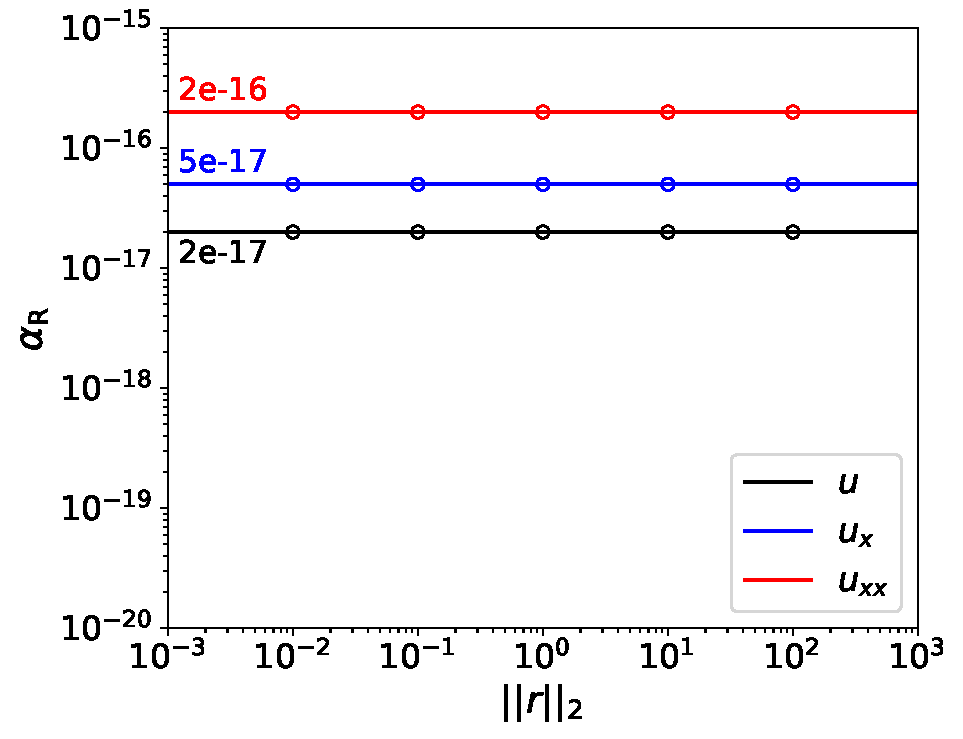
\includegraphics[width=1.0\linewidth]{../2_figure/4_offset_summary/py_offset_summary_Helm_sm.pdf}
        \caption{The standard FEM}
        \label{py_offset_summary_Helm_sm}
    \end{subfigure}
    \hspace{-0.2cm}
    \begin{subfigure}{6.0cm}
        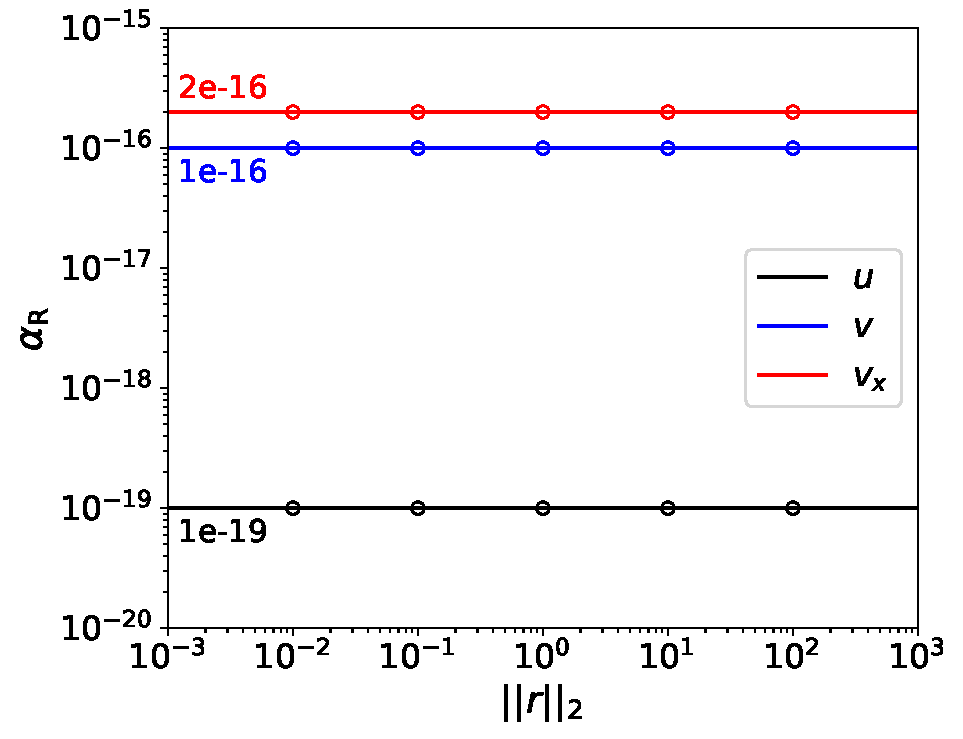
\includegraphics[width=1.0\linewidth]{../2_figure/4_offset_summary/py_offset_summary_Helm_mm.pdf}
        \caption{The mixed FEM}
        \label{py_offset_summary_Helm_mm}
    \end{subfigure}
\caption{$\alpha_{\rm R}$ for the general Helmholtz equations.}
\label{py_offset_summary_Helm}
\end{figure}

In Figs. \ref{py_offset_summary_diff}--\ref{py_offset_summary_Helm}, we do not take the influence of $\|u\|_2$ or$\|v\|_2$ into account. Since $\|u\|_2$ is of order 1, we omit its influence on $\alpha_{\rm R}$ for the standard FEM and on $\alpha_{\rm R}$ of $u$ and $v$ for the mixed FEM. Since $\|v\|_2$ is half of 1, we multiply the intercept of $\alpha_{\rm R}$ of $v_x$ in Fig. \ref{py_offset_summary_diff_mm} and the upper bound of $\alpha_{\rm R}$ of $v_x$ in Fig. \ref{py_offset_summary_Helm_mm} by 2, for validating the constant term of $\alpha_{\rm R}$ in Table \ref{relation_alpha_R_l2_norm}.

Comparing the resulting $\alpha_{\rm R}$ of the diffusion equations with the constant term of $\alpha_{\rm R}$ in Table \ref{relation_alpha_R_l2_norm}, for the standard FEM, the constant term of $\alpha_{\rm R}$ of $u$ and $u_x$ does not change, while that of $u_{xx}$ increases to 1e-15; for the mixed FEM, the constant term of $\alpha_{\rm R}$ of $u$ increases to 5e-17, that of $v$ becomes 2e-16 $\times \|d\|_2$, and that of $v_x$ increases to 1e-15. Therefore, we amend $\alpha_{\rm R}$ in Table \ref{relation_alpha_R_l2_norm} to be that shown in Table~\ref{relation_alpha_R_l2_norm_amended}. Note that, for the constant term of $\alpha_{\rm R}$ of $u$ of the mixed FEM, considering most of its values of the diffusion equations are smaller than 2e-17, which is the value we obtain for the standard FEM, we choose 2e-17 as its value. Furthermore, since the constant term of $\alpha_{\rm R}$ of the Helmholtz equations is smaller than that in Table \ref{relation_alpha_R_l2_norm_amended}, its effect can be ignored.


\begin{table}[!ht]
\small
\captionof{table}{$\alpha_{\rm R}$ in terms of the product of a constant and the $L_2$ norm $\|u\|_2$ or $\|v\|_2$, dependent on the specific dependent variable, for one-dimensional second order differential equations.}
\hspace{3.0cm}
\begin{subtable}{0.4\textwidth}
\caption{The standard FEM}
\label{relation_alpha_R_l2_norm_amended_std}
\begin{tabular}{c | l c}
\hline
Variable & \multicolumn{2}{c}{$\alpha_{\rm R}$} \\ \hline
$u$ & 2e-17 & \multirow{3}{*}{$\Bigg\}\times \|u\|_2$} \\ \cline{1-2}
$u_x$ & 5e-17 & \\ \cline{1-2}
$u_{xx}$ & 1e-15 & \\ \hline
\end{tabular}
\end{subtable}
\hspace{-2cm}
\begin{subtable}{.4\textwidth}
\caption{The mixed FEM}
\label{relation_alpha_R_l2_norm_amended_mix}
\begin{tabular}{c | l c}
\hline
Variable & \multicolumn{2}{c}{$\alpha_{\rm R}$} \\ \hline
$u$ & 2e-17 & \multirow{2}{*}{$\bigg\}\times\|u\|_2$} \\ \cline{1-2} 
$v$ & 2e-16 $\times \|d\|_2$ &  \\ \hline
$v_x$ & 1e-15 & $\times \|v\|_2$ \\ \hline
\end{tabular}
\end{subtable}
\label{relation_alpha_R_l2_norm_amended}
\end{table}

Summarizing Sections \ref{section_general_poisson} -- \ref{section_d_and_r}, the order of magnitude of the coefficient $r(x)$ is basically irrelevant; the order of magnitude of the dependent variable and the coefficient $d(x)$ can be mitigated when their values are known. Specifically, the value of the order of magnitude of the dependent variable can be obtained from a built-in function in our algorithm, and that of $d(x)$ can be obtained by carrying out simple integration.

%\newpage
\section{A posteriori algorithm for finding the optimal number of degrees of freedom}		\label{section_algorithm}

Based on the validation experiments from the previous section, we introduce a novel a posteriori algorithm for determining $E_{\rm min}$ and its associated $N_{\rm opt}$ for the solution and its first and second derivative without performing brute-force mesh refinement. We call the algorithm $DoFinder$.

In $DoFinder$, we define the following coefficients and use them in the steps given below.

\begin{itemize}
  \renewcommand\labelitemi{--}
  \item a minimal number of $h$-refinements before carrying out `\textit{NORMALIZATION}' and `\textit{PREDICTION}', denoted by $R_{\rm min}$, with the following default values:
  \begin{equation}
  \begin{aligned}
      R_{\rm min} &=
      \begin{cases*}
	9-p & for $p < 6$, \\
	4 & otherwise.
      \end{cases*}
  \end{aligned}
  \end{equation}
  We choose this parameter mainly because the error might increase, or decrease faster than the asymptotic order of convergence for coarse refinements, especially for lower-order elements.
  \item the allowed maximum $N_h$ : $10^8$, denoted by $N_{\rm max}$.  
  \item a stopping criterion $c_s$ for seeking the $L_2$ norm of the dependent variable, of which the value is 0.001 by default. We choose this parameter because the analytical solution does not exist for most practical problems.
  \item a relaxation coefficient $c_r$ for seeking the asymptotic order of convergence, with the following default values: 
    \begin{equation}
    \begin{aligned}
	c_r &=
	\begin{cases*}
	  0.9 & for $p<4$, \\
	  0.7 & for 4 $\leqslant$ $p < 10$, \\
	  0.5 & otherwise.
	\end{cases*}
    \end{aligned}
    \end{equation}
  \item the offset $\alpha _{\rm R}$, see Table \ref{relation_alpha_R_l2_norm_amended} for the default values.
\end{itemize}

% \newpage
The procedure of $DoFinder$ consists of four steps, which are explained below:

\paragraph{Step-1} `\textit{INPUT}'. In this step, the custom input shown in the Table \ref{settings_algorithm} has to be provided.

\begin{table}[!ht]
\small
\captionof{table}{Custom input of $DoFinder$.}
\label{settings_algorithm}
  \centering
  \begin{tabular}{l | L{10cm}}
    \toprule
    Type & Item  \\
    \midrule
    Problem & \tabitem the differential equation to be solved \\
     		& \tabitem variables of interest \\ \hline
    FEM     & \tabitem standard or mixed formulation \\
    		& \tabitem an ordered array of element degrees $\{p_{\min}, \ldots, p_{\rm max}\}$ \\
    \bottomrule
  \end{tabular}
\end{table}

\paragraph{Step-2} `\textit{NORMALIZATION}'. The function of this step is to find the $L_2$ norm of the dependent variable, in which elements of degree $p_{\rm min}$ are used. The specific procedure can be found in Algorithm \ref{algo_scaling_factor}. 

\vspace{0.2cm}
\begin{algorithm}[H]
\caption{NORMALIZATION}
\label{algo_scaling_factor}
\While{$N_h<N_{\rm max}$}
{
    \eIf{$\left|\frac{\|var_{h}\|_{2} - \|var_{2h}\|_{2}}{\|var_{h}\|_{2}} \right| < c_s$}
    {
        $\|var\|_{2}$ $\gets$ $\|var_{h}\|_{2}$\;
        break\;
    }
    {
        $h$ $\gets$ $h/2$\;
        calculate $\|var_h\|_{2}$\;    
    }
}
\end{algorithm}
                                                                   
\paragraph{Step-3} `\textit{PREDICTION}'. This step finds $E_{\rm min}$ for each $var$ and $p$ of interest, as illustrated in Fig.~\ref{error_evolution_one_p}.
The procedure for carrying out this step can be found in Algorithm \ref{block_PREDICTION}.

\vspace{0.2cm}
\begin{algorithm}[H]
\caption{PREDICTION}			% Seeking the analytical order of convergence Predicting $N_{\rm opt}$ and $E_{\rm min}$
\label{block_PREDICTION}
    \While{$N_h<N_{\rm max}$ \textbf{\textup{and}} $\widetilde {E_{h}}>E_{\rm R}$}
    {
        $\widetilde{Q}$ $\gets$ $\log _2 \left( {\widetilde {E_{2h}}}/{\widetilde {E_{h}}} \right)$\;
        \eIf
        {
            $\widetilde{Q} \geqslant \beta_{\rm T} \times c_r$
        }
        {
            $N_{\rm c} \gets N_h$\;
            $E_{\rm c} \gets \widetilde {E_{h}}$\;
            $\alpha_{\rm T}$ $\gets$ ${E_{\rm c}}/{N_{\rm c}}^{- \beta_{\rm T}}$\;
            $N_{\rm opt} \gets \left( \frac{\alpha_{\rm T} \beta_{\rm T}}{\alpha _{\rm R} \beta_{\rm R}} \right)^{\frac{1}{\beta_{\rm R} + \beta_{\rm T}}}$\;
            $E_{\rm min} \gets \alpha_{\rm T} {N_{\rm opt}}^{- {\beta _{\rm T}}} + \alpha_{\rm R} {N_{\rm opt}}^{{\beta _{\rm R}}}$\;

        }
        {
            $h$ $\gets$ $h/2$\;
            calculate $\widetilde {E_{h}}$\;
        }
	}    
\end{algorithm}

\paragraph{Step-4} `\textit{OUTPUT}'. In this step, we output $E_{\rm min}$, $N_{\rm opt}$, etc., obtained from \textit{Step-3}.

\section{Validation}		\label{section_validation}

In what follows, we validate the strategy discussed in Section \ref{section_error_evolution_and_prediction} by using the following Helmholtz problem:
\begin{equation}
  \left((0.01+x)(1.01-x) u_x \right)_x -(0.01i) u(x) = 1.0,\qquad x \in I = [0,1],	\label{1D_Helmholtz_equation_application}
\end{equation}
with homogeneous Dirichlet and Neumann boundary conditions imposed as follows: $u(0)=0$ and $u_x(1)=0$.
Both the standard FEM and the mixed FEM are investigated, with the element degree $p$ taken in $\{1, 2, \ldots, 5\}$. Variables $u$, $u_x$ and $u_{xx}$ using the standard FEM and $u$, $v$ and $v_x$ using the mixed FEM are investigated.

\subsection{Accuracy analysis}					\label{section_accuracy_analysis}
Using $DoFinder$ and the brute-force approach, $E_{\rm min}$'s are compared in Fig.~\ref{E_min_application}. As can be seen, $E_{\rm min}$ can be predicted correctly. Note that, for $p=1$ using the mixed FEM, we cannot obtain $E_{\rm min}$ of the brute-force approach because of the limited hardware. The associated $N_{\rm opt}$ using $DoFinder$ is shown in Fig.~\ref{N_opt_application}, and it is used to compute the solution of the optimal grid in Section \ref{section_efficiency_analysis}.

\begin{figure}[!ht]
	\centering
    \begin{subfigure}{6.0cm}
        \includegraphics[width=1.0\linewidth]{../2_figure/8_algorithm_plot/py_comparison_DoFinder_accuracy_sm.pdf}
        \caption{The standard FEM}
        \label{E_min_application_sm}
    \end{subfigure}
    \begin{subfigure}{6.0cm}	                		 	
        \includegraphics[width=1.0\linewidth]{../2_figure/8_algorithm_plot/py_comparison_DoFinder_accuracy_mm.pdf}
        \caption{The mixed FEM}
        \label{E_min_application_mm}
    \end{subfigure}
\caption{$E_{\rm min}$ for Eq. (\ref{1D_Helmholtz_equation_application}) using $DoFinder$. The filled circle denotes results using the brute-force approach.}
\label{E_min_application}
\end{figure}

\begin{figure}[!ht]
	\centering
    \begin{subfigure}{6.0cm}
        \includegraphics[width=1.0\linewidth]{../2_figure/8_algorithm_plot/py_comparison_DoFinder_n_opt_sm.pdf}
        \caption{The standard FEM}
        \label{N_opt_application_sm}
    \end{subfigure}
    \begin{subfigure}{6.0cm}	                		 	
        \includegraphics[width=1.0\linewidth]{../2_figure/8_algorithm_plot/py_comparison_DoFinder_n_opt_mm.pdf}
        \caption{The mixed FEM}
        \label{N_opt_application_mm}
    \end{subfigure}
\caption{$N_{\rm opt}$ for Eq. (\ref{1D_Helmholtz_equation_application}) using $DoFinder$.}
\label{N_opt_application}
\end{figure}

%\newpage
\subsection{Efficiency analysis}				\label{section_efficiency_analysis}

The CPU time required by $DoFinder$ and the brute-force approach is shown in Fig.~\ref{CPU_brut} and Fig.~\ref{CPU_pred_only}, respectively. In general, the CPU time associated with the brute-force approach decreases with increasing element degree. In comparison with the CPU time of the brute-force approach, the CPU time of $DoFinder$ is negligible.

\begin{figure}[!ht]
	\centering
    \begin{subfigure}{6.0cm}
        \includegraphics[width=1.0\linewidth]{../2_figure/8_algorithm_plot/py_comparison_DoFinder_cpu_brut_sm.pdf}
        \caption{The standard FEM}
        \label{CPU_brut_sm}
    \end{subfigure}
    \begin{subfigure}{6.0cm}	                		 	
        \includegraphics[width=1.0\linewidth]{../2_figure/8_algorithm_plot/py_comparison_DoFinder_cpu_brut_mm.pdf}
        \caption{The mixed FEM}
        \label{CPU_brut_mm}
    \end{subfigure}
\caption{CPU time required by the brute-force approach to obtain $E_{\rm min}$ for Eq. (\ref{1D_Helmholtz_equation_application}).}
\label{CPU_brut}
\end{figure}

\begin{figure}[!ht]
	\centering
    \begin{subfigure}{6.0cm}
        \includegraphics[width=1.0\linewidth]{../2_figure/8_algorithm_plot/py_comparison_DoFinder_cpu_pred_only_sm.pdf}
        \caption{The standard FEM}
        \label{CPU_pred_only_sm}
    \end{subfigure}
    \begin{subfigure}{6.0cm}	                		 	
        \includegraphics[width=1.0\linewidth]{../2_figure/8_algorithm_plot/py_comparison_DoFinder_cpu_pred_only_mm.pdf}
        \caption{The mixed FEM}
        \label{CPU_pred_only_mm}
    \end{subfigure}
\caption{CPU time required by $DoFinder$ to obtain $E_{\rm min}$ for Eq. (\ref{1D_Helmholtz_equation_application}).}
\label{CPU_pred_only}
\end{figure}

Furthermore, to obtain the solution on the optimal grid based on $DoFinder$, the computation time can be saved much in comparison with that using the brute-force approach. Fig.~\ref{CPU_saved} gives the percentage of the CPU time saved by $DoFinder$. It shows a saving of the CPU time of around 70\% for both the standard FEM and the mixed FEM. 

\begin{figure}[!ht]
	\centering
    \begin{subfigure}{6.0cm}
        \includegraphics[width=1.0\linewidth]{../2_figure/8_algorithm_plot/py_comparison_DoFinder_cpu_saved_sm.pdf}
        \caption{The standard FEM}
        \label{CPU_saved_sm}
    \end{subfigure}
    \begin{subfigure}{6.0cm}	                		 	
        \includegraphics[width=1.0\linewidth]{../2_figure/8_algorithm_plot/py_comparison_DoFinder_cpu_saved_mm.pdf}
        \caption{The mixed FEM}
        \label{CPU_saved_mm}
    \end{subfigure}
\caption{Percentage of CPU time saved by $DoFinder$ to obtain $E_{\rm min}$ for Eq. (\ref{1D_Helmholtz_equation_application}).}
\label{CPU_saved}
\end{figure}

%\newpage
\subsection{Further development}						\label{section_further_development}

For a given tolerance of a variable, denoted by $tol_{var}$, we are able to quickly select the available FEM method, the associated minimal available $p$ and minimal available number of DoFs. For example, when $tol_{u}=1$e-9, we can only achieve it using the mixed FEM, the associated minimal available $p$ is 2, and minimal available number of DoFs is 638876.

\section{Conclusions}		\label{paragraph on conclusion}

A novel approach is presented to predict the highest attainable accuracy for second order, ordinary differential equations using the finite element method.
In contrast to the brute-force approach, which uses successive $h$-refinements, this approach uses only a few coarse grid refinements to reach the region of asymptotic convergence. 
This approach is viable for the solution and its first and second derivative, for both the standard FEM and the mixed FEM, for all element degrees.
The algorithm for implementing the approach shows that the highest attainable accuracy can be accurately predicted using negligible CPU time and the CPU time to obtain this solution explicitly is significantly reduced: to compute the solution with the highest attainable accuracy using our approach results in a reduction of CPU time by around 70\% for both the standard FEM and  the mixed FEM.
Future research will focus on the extension of this approach to 2D second order problems, where the influence of the linear system solver, local mesh refinement and boundary conditions might be significantly different from 1D problems. 

\appendix

\section{Derivation of the weak form}		\label{weak form appendix}

\subsection{The standard FEM}		\label{derivation_weak_form_SM}

Multiply Eq. (\ref{1d_second_order_differential_equation}) by a test function $\eta \in H ^1 (I)$, and integrate it over $I$ yield
\begin{equation}
\langle \eta, \, -\left( d u_x \right)_x + ru \rangle = \langle \eta, \, f \rangle. \label{sm_weak_form_inte}
\end{equation}
By applying Gauss's theorem, we obtain
\begin{equation}
 \langle {\eta} _x, \, d u_x \rangle + \langle \eta, \, ru \rangle = \langle \eta, \, f \rangle + \langle \eta, \, d u_x n \rangle_{ {\Gamma}}.		\label{sm_weak_form_gauss}
\end{equation}
Substituting the natural boundary conditions, i.e. $d(x)u_x=h(x)$ on $\Gamma_N$, and taking $\eta=0$ on $\Gamma_{D}$ render Eq.~({\ref{sm_weak_form_Diri_strong}}); substituting the natural boundary conditions, not taking $\eta=0$ on $\Gamma_{D}$, but adding auxiliary terms render Eq. (\ref{sm_weak_form_Diri_weak}).

\subsection{The mixed FEM}		\label{derivation_weak_form_MM}
Multiply Eq. (\ref{mm_strong_form_1}) by a test function of $v$, i.e. $w \in H _{N0}^{1}(I)$, and integrate it over $I$ yield
\begin{subequations}
\begin{align}
  \langle d^{-1}v + u _x, w \rangle = 0.	\label{mm_weak_form_1_inte}
\end{align}
Applying Gauss's theorem to Eq.~(\ref{mm_weak_form_1_inte}), it becomes
\begin{align}
 \langle w, \, d^{-1}v \rangle - \langle w_x, \,  u \rangle = -\langle w, \, u n\rangle_{\Gamma _D}.		\label{mm_weak_form_1_gauss}
\end{align}%
\end{subequations}
Substituting the natural boundary conditions, i.e. $u(x)=g(x)$ on $\Gamma_D$, renders Eq.~({\ref{mm_weak_form_1}}). Note that, unlike the standard FEM, the essential boundary conditions are imposed on $\Gamma _N$ and the natural boundary conditions are imposed on $\Gamma _D$ for the mixed FEM.

Multiply Eq. (\ref{mm_strong_form_2}) by a test function of $u$, i.e. $q \in L^2 (I)$, and integrate it over $I$ yield
\begin{align}
- \langle q , \, v_x \rangle - \langle q, \, ru \rangle = - \langle q, \, f \rangle,
\end{align}
which results in Eq.~(\ref{mm_weak_form_2}).

\section{Proof of the slope of the decrease of the error}				\label{proof_slope_ET}

Here we give the proof for the standard FEM. The process for the mixed FEM is similar. 

For the grid size $h$ and element degree $p$, the number of DoFs
\begin{equation}
N_h=(1/h) \times p+1.			\label{formula_Nh}
\end{equation}
Therefore,
\begin{equation}
h=\frac{p}{N_h-1}.		\label{formula_h}
\end{equation}
Since the error \cite{gockenbach2006understanding}
\begin{equation}
E_h \leqslant Ch^{p+1},			\label{formula_Eh_with_h}
\end{equation}
substituting Eq.~(\ref{formula_h}) into Eq.~(\ref{formula_Eh_with_h}), we obtain
\begin{equation}
E_h \leqslant C_1(N_h-1)^{-(p+1)},			\label{formula_Eh_with_Nh}
\end{equation}
where $C_1=C p^{p+1}$. Therefore, the slope is $\beta_{\rm T}=p+1$

\bibliographystyle{unsrt}  
\bibliography{mybibfile}


\end{document}
